\documentclass{ieeeaccess}

\usepackage{cite}
\usepackage{amsmath,amssymb,amsfonts}
\usepackage{mathtools}
\usepackage{algorithm}
\usepackage{algorithmic}
\usepackage{graphicx}
\usepackage{textcomp}
\usepackage{booktabs}
\usepackage{multirow}
\usepackage{array}
\usepackage{url}
\usepackage{dcolumn}
\usepackage{float}
\usepackage[hidelinks]{hyperref}

\usepackage{bm}
\makeatletter
\AtBeginDocument{\DeclareMathVersion{bold}
\SetSymbolFont{operators}{bold}{T1}{times}{b}{n}
\SetSymbolFont{NewLetters}{bold}{T1}{times}{b}{it}
\SetMathAlphabet{\mathrm}{bold}{T1}{times}{b}{n}
\SetMathAlphabet{\mathit}{bold}{T1}{times}{b}{it}
\SetMathAlphabet{\mathbf}{bold}{T1}{times}{b}{n}
\SetMathAlphabet{\mathtt}{bold}{OT1}{pcr}{b}{n}
\SetSymbolFont{symbols}{bold}{OMS}{cmsy}{b}{n}
\renewcommand\boldmath{\@nomath\boldmath\mathversion{bold}}}
\makeatother

% ---------------------------------------------------------------------
% Placeholder macros for headline numbers. They are filled in by
% scripts via search-and-replace once the walk-forward,
% ablation, risk-metrics, regime-analysis, cost-sensitivity, and
% correlation scripts have completed.
% ---------------------------------------------------------------------
% Headline metrics and bootstrap CIs
\newcommand{\TRtrain}{\ensuremath{0.55}}
\newcommand{\TRtest}{\ensuremath{0.23}}
\newcommand{\TRtestCIlow}{\ensuremath{-0.10}}
\newcommand{\TRtestCIhigh}{\ensuremath{0.68}}
\newcommand{\Shtest}{\ensuremath{1.06}}
\newcommand{\ShtestCIlow}{\ensuremath{-0.43}}
\newcommand{\ShtestCIhigh}{\ensuremath{2.57}}
\newcommand{\MDDtest}{\ensuremath{-0.06}}
\newcommand{\Calmtest}{\ensuremath{2.10}}
\newcommand{\CAGRtest}{\ensuremath{0.13}}
\newcommand{\Ntrades}{\ensuremath{34}}
\newcommand{\WinRate}{\ensuremath{0.65}}
\newcommand{\BHtest}{\ensuremath{0.31}}
\newcommand{\BHsharpe}{\ensuremath{0.82}}
\newcommand{\MDDbh}{\ensuremath{-0.17}}
\newcommand{\CAGRbh}{\ensuremath{0.17}}
\newcommand{\Calmbh}{\ensuremath{0.96}}
\newcommand{\PvsBH}{\ensuremath{0.636}}
\newcommand{\PvsBHsharpe}{\ensuremath{0.297}}
\newcommand{\BestSingleName}{\texttt{only\_rsi}}
\newcommand{\BestSingleTR}{\ensuremath{0.16}}
\newcommand{\PvsBestSingle}{\ensuremath{0.268}}
\newcommand{\BestMode}{\texttt{aggressive}}
\newcommand{\BestMinConf}{\ensuremath{0.05}}
% Risk-adjusted metrics (OOS, net of costs)
\newcommand{\EnsSortino}{\ensuremath{1.60}}
\newcommand{\BHSortino}{\ensuremath{1.19}}
\newcommand{\EnsDownDev}{\ensuremath{0.08}}
\newcommand{\BHDownDev}{\ensuremath{0.15}}
\newcommand{\EnsUlcer}{\ensuremath{2.39}}
\newcommand{\BHUlcer}{\ensuremath{6.69}}
\newcommand{\EnsMartin}{\ensuremath{5.29}}
\newcommand{\BHMartin}{\ensuremath{2.49}}
% Volatility-matched comparison
\newcommand{\VolScaledTR}{\ensuremath{0.49}}
\newcommand{\VolScaledCAGR}{\ensuremath{0.26}}
\newcommand{\VolScaledSharpe}{\ensuremath{1.06}}
\newcommand{\VolScaledMDD}{\ensuremath{-0.12}}
\newcommand{\VolScaledCalmar}{\ensuremath{2.13}}
\newcommand{\VolScaledSortino}{\ensuremath{1.63}}
\newcommand{\VolScaledUlcer}{\ensuremath{4.96}}
\newcommand{\Leverage}{\ensuremath{2.06}}
\newcommand{\StrategyTrainVol}{\ensuremath{0.11}}
\newcommand{\BHOosVol}{\ensuremath{0.22}}
\newcommand{\VolScaledExcessPP}{\ensuremath{+18.55}}
% Regime decomposition
\newcommand{\OOSDays}{\ensuremath{435}}
\newcommand{\RegBullDays}{\ensuremath{230}}
\newcommand{\RegCorrectionDays}{\ensuremath{93}}
\newcommand{\RegSidewaysDays}{\ensuremath{112}}
\newcommand{\RegBullShare}{52.87\%}
\newcommand{\RegCorrectionShare}{21.38\%}
\newcommand{\RegSidewaysShare}{25.75\%}
\newcommand{\EnsBullTR}{\ensuremath{0.26}}
\newcommand{\EnsBullSharpe}{\ensuremath{2.47}}
\newcommand{\EnsCorrectionTR}{\ensuremath{-0.07}}
\newcommand{\EnsCorrectionSharpe}{\ensuremath{-1.34}}
\newcommand{\EnsSidewaysTR}{\ensuremath{0.05}}
\newcommand{\EnsSidewaysSharpe}{\ensuremath{0.93}}
\newcommand{\EnsAllTR}{\ensuremath{0.23}}
\newcommand{\EnsAllSharpe}{\ensuremath{1.06}}
\newcommand{\BHBullTR}{\ensuremath{0.63}}
\newcommand{\BHBullSharpe}{\ensuremath{2.76}}
\newcommand{\BHCorrectionTR}{\ensuremath{-0.20}}
\newcommand{\BHCorrectionSharpe}{\ensuremath{-2.41}}
\newcommand{\BHSidewaysTR}{\ensuremath{-0.00}}
\newcommand{\BHSidewaysSharpe}{\ensuremath{0.11}}
\newcommand{\BHAllTR}{\ensuremath{0.31}}
\newcommand{\BHAllSharpe}{\ensuremath{0.82}}
\newcommand{\CorrectionDefencePP}{\ensuremath{+12.57}}
\newcommand{\SidewaysExcessPP}{\ensuremath{+5.14}}
\newcommand{\BullShortfallPP}{\ensuremath{-36.84}}
% Cost sensitivity
\newcommand{\CostZeroTR}{\ensuremath{0.25}}
\newcommand{\CostZeroSharpe}{\ensuremath{1.15}}
\newcommand{\CostBaseTR}{\ensuremath{0.23}}
\newcommand{\CostBaseSharpe}{\ensuremath{1.06}}
\newcommand{\CostWorstTR}{\ensuremath{0.20}}
\newcommand{\CostWorstSharpe}{\ensuremath{0.92}}
\newcommand{\CostMinSharpe}{\ensuremath{0.92}}
% Agent signal correlations
\newcommand{\CorrMeanAbs}{\ensuremath{0.25}}
\newcommand{\CorrMin}{\ensuremath{-0.71}}
\newcommand{\CorrMax}{\ensuremath{0.46}}
\newcommand{\CorrN}{\ensuremath{10}}
% Deep-learning (LSTM) baseline on WIG20
\newcommand{\LSTMtest}{\ensuremath{0.08}}
\newcommand{\LSTMsharpe}{\ensuremath{0.44}}
\newcommand{\LSTMmdd}{\ensuremath{-0.11}}
\newcommand{\LSTMcalmar}{\ensuremath{0.42}}
\newcommand{\LSTMtrades}{\ensuremath{237}}
\newcommand{\LSTMhorizon}{\ensuremath{3}}
\newcommand{\LSTMband}{\ensuremath{0.03}}
\newcommand{\PensVsLSTM}{\ensuremath{0.068}}
\newcommand{\PensVsLSTMsharpe}{\ensuremath{0.063}}
% External validation on the FTSE 100
\newcommand{\FtseNsymbols}{\ensuremath{20}}
\newcommand{\FtseOOSDays}{\ensuremath{444}}
\newcommand{\FtseTRtest}{\ensuremath{0.14}}
\newcommand{\FtseCAGR}{\ensuremath{0.08}}
\newcommand{\FtseMDD}{\ensuremath{-0.07}}
\newcommand{\FtseSharpe}{\ensuremath{1.37}}
\newcommand{\FtseCalmar}{\ensuremath{1.18}}
\newcommand{\FtseNtrades}{\ensuremath{55}}
\newcommand{\FtseWinRate}{\ensuremath{0.78}}
\newcommand{\FtseTRtestCIlow}{\ensuremath{-0.01}}
\newcommand{\FtseTRtestCIhigh}{\ensuremath{0.32}}
\newcommand{\FtseSharpeCIlow}{\ensuremath{-0.11}}
\newcommand{\FtseSharpeCIhigh}{\ensuremath{2.94}}
\newcommand{\FtseBHtest}{\ensuremath{0.25}}
\newcommand{\FtseBHcagr}{\ensuremath{0.13}}
\newcommand{\FtseBHmdd}{\ensuremath{-0.13}}
\newcommand{\FtseBHsharpe}{\ensuremath{1.13}}
\newcommand{\FtseBHcalmar}{\ensuremath{1.00}}
\newcommand{\FtsePvsBH}{\ensuremath{0.789}}
\newcommand{\FtsePvsBHsharpe}{\ensuremath{0.331}}
\newcommand{\FtseEnsSortino}{\ensuremath{1.99}}
\newcommand{\FtseBHSortino}{\ensuremath{1.52}}
\newcommand{\FtseEnsDownDev}{\ensuremath{0.04}}
\newcommand{\FtseBHDownDev}{\ensuremath{0.09}}
\newcommand{\FtseEnsUlcer}{\ensuremath{1.59}}
\newcommand{\FtseBHUlcer}{\ensuremath{2.66}}
\newcommand{\FtseEnsMartin}{\ensuremath{4.91}}
\newcommand{\FtseBHMartin}{\ensuremath{5.05}}
\newcommand{\FtseLeverage}{\ensuremath{1.82}}
\newcommand{\FtseVolScaledTR}{\ensuremath{0.26}}
\newcommand{\FtseVolScaledSharpe}{\ensuremath{1.37}}
\newcommand{\FtseVolScaledMDD}{\ensuremath{-0.12}}
\newcommand{\FtseVolScaledExcessPP}{\ensuremath{+1.87}}
\newcommand{\FtseRegBullShare}{90.32\%}
\newcommand{\FtseRegBullDays}{\ensuremath{401}}
\newcommand{\FtseRegCorrectionDays}{\ensuremath{5}}
\newcommand{\FtseRegSidewaysDays}{\ensuremath{38}}
\newcommand{\FtseEnsBullTR}{\ensuremath{0.14}}
\newcommand{\FtseBHBullTR}{\ensuremath{0.30}}
\newcommand{\FtseEnsCorrectionTR}{\ensuremath{-0.02}}
\newcommand{\FtseBHCorrectionTR}{\ensuremath{-0.01}}
\newcommand{\FtseEnsSidewaysTR}{\ensuremath{0.02}}
\newcommand{\FtseBHSidewaysTR}{\ensuremath{-0.03}}
\newcommand{\FtseBestSingleName}{\texttt{only\_macd}}
\newcommand{\FtseBestSingleTR}{\ensuremath{0.15}}
\newcommand{\FtseLSTMtest}{\ensuremath{0.27}}
\newcommand{\FtseLSTMsharpe}{\ensuremath{1.49}}
\newcommand{\FtseLSTMmdd}{\ensuremath{-0.08}}
\newcommand{\FtseLSTMtrades}{\ensuremath{37}}
\newcommand{\FtsePensVsLSTM}{\ensuremath{0.879}}
\newcommand{\FtsePLSTMvsBH}{\ensuremath{0.411}}

% ---------------------------------------------------------------------

\begin{document}

%\history{Date of submission April XX, 2026.}
%\doi{}

\title{A Risk-Aware Multi-Agent Decision Support System for Stock Trading on the Warsaw Stock Exchange: A Forecast-Combination Approach with Walk-Forward Evaluation}

\author{\uppercase{Rafal Jankowski}\authorrefmark{1},
\uppercase{Pawel Weichbroth}\authorrefmark{2}}

\address[1]{Faculty of Electronics, Telecommunications, and Informatics, Gdańsk University of Technology, 80-233 Gdańsk, Poland}
\address[2]{Faculty of Electronics, Telecommunications, and Informatics, Gdańsk University of Technology, 80-233 Gdańsk, Poland}

\tfootnote{The source code and data-preparation scripts used in this study are available upon reasonable request.}

\markboth
{Jankowski, Weichbroth: Risk-Aware Multi-Agent Decision Support System for Stock Trading}
{Jankowski, Weichbroth: Risk-Aware Multi-Agent Decision Support System for Stock Trading}

\corresp{Corresponding author: Paweł Weichbroth (e-mail: pawel.weichbroth@pg.edu.pl).}

\begin{abstract}
We present a multi-agent decision support system for stock trading on the Warsaw Stock Exchange (WSE), a Central and Eastern European market underrepresented in the algorithmic trading literature. The system aggregates signals from five signal agents through a configurable decision agent. The design is grounded in forecast-combination theory, which predicts variance reduction when several imperfect forecasters are combined. The evaluation addresses four common weaknesses of backtested trading studies: in-sample parameter selection, absent transaction costs, neglect of risk-adjusted performance, and lack of significance tests. An anchored walk-forward protocol tunes only the decision-agent parameters, a calibrated commission and slippage model is applied to every trade, and risk-adjusted performance is summarized with the Sharpe, Sortino, Calmar, and Martin ratios and the Ulcer Index, with a volatility-matched comparison and bootstrap confidence intervals on headline claims. On the held-out test window for the twenty-stock blue-chip index WIG20, over \OOSDays{} trading days across bull, correction, and sideways regimes, the ensemble underperforms passive buy-and-hold on raw total return over the bull-dominated subperiod, but materially outperforms it on every risk-adjusted metric considered and, once both series are scaled to the same ex-ante volatility, also on total return. A regime decomposition shows smaller losses during corrections and higher returns during sideways phases, offset by lower bull-market returns. Cost-sensitivity and ablation checks confirm robustness. The results support theory-grounded ensembles as risk-aware decision support rather than return enhancers.
\end{abstract}

\begin{keywords}
Algorithmic trading, decision support systems, forecast combination, multi-agent systems, risk-adjusted performance, walk-forward validation, Warsaw Stock Exchange.
\end{keywords}

\titlepgskip=-21pt

\maketitle

% ==============================================================================
\section{Introduction}
\label{sec:introduction}
% ==============================================================================
\PARstart{D}{ecision} support systems and algorithmic trading occupy a central place in contemporary financial markets. They help both institutional and retail investors process large volumes of market information and translate that information into trading actions \cite{hendershott_does_2011}. Over the last two decades, research on algorithmic trading has expanded from simple rule-based strategies \cite{brock1992} to machine-learning classifiers \cite{gerlein2016,fischerkrauss2018}, and more recently to deep reinforcement learning systems that learn trading policies directly from data \cite{huang2022,shavandi2022,kaursingh2023}. In parallel, multi-agent systems (MAS) have been proposed as a natural way to organize this diversity of trading rules and models, so that independent agents can produce signals that a coordinator combines into the final decision \cite{luo2002,korczak2013,hernes2016,hernes2024}.

Despite the breadth of this literature, four methodological weaknesses recur in empirical studies of trading strategies. The first is \emph{in-sample parameter selection}: when the best configuration of a strategy is chosen on the same data used to evaluate it, the out-of-sample performance is overstated \cite{bailey2014,harvey2016}. The second is the \emph{omission of realistic frictions}, in particular commissions and slippage, which can erode a noticeable fraction of the gross return of high-turnover configurations. The third is the \emph{neglect of risk-adjusted performance}: many studies compare a trading strategy to passive buy-and-hold purely on cumulative profit, without taking into consideration that an active strategy can produce a smoother equity curve at a lower unleveraged return. This weakness is particularly acute during sustained bull markets, where passive exposure mechanically dominates any strategy that is occasionally out of the market \cite{dichtl2020}. The fourth is the \emph{absence of formal significance tests}: headline metrics are often reported as point estimates without confidence intervals or paired tests against the benchmark, even though trading-strategy metrics are known to be non-Gaussian and path-dependent \cite{politis1994,bailey2014}. Beyond these methodological issues, the empirical evidence on multi-agent decision support systems is strongly concentrated on major markets in the United States, Western Europe, and Asia; the Warsaw Stock Exchange (WSE)---the largest exchange in Central and Eastern Europe (CEE) by capitalization---has received much less attention \cite{czapkiewicz2015,jagric2015,buczynski2021}.

The present paper addresses these four methodological weaknesses in combination, on a market that has received limited attention. First, it proposes a multi-agent decision support system for WIG20 stocks that aggregates five heterogeneous signal agents through a transparent decision agent. The aggregator is interpreted through the lens of forecast-combination theory \cite{batesgranger1969,clemen1989,timmermann2006}: each signal agent is treated as an imperfect forecaster of the next-period directional move, and the per-signal confidence value is interpreted as a monotone proxy for the inverse variance of that forecaster at that point in time. Second, the evaluation follows an anchored walk-forward protocol in which only the decision-agent parameters are tuned on training data, whereas indicator hyperparameters are fixed at their literature-conventional values and all headline metrics are reported on a held-out test window that is never seen during parameter selection. Third, all backtests include a proportional commission and one-way slippage calibrated to typical Polish retail brokerage conditions, and both quantities are swept over a grid to quantify cost sensitivity. Fourth, the evaluation is centered on \emph{risk-adjusted} performance rather than on gross total return: we report Sharpe, Sortino, Calmar, and Martin ratios, and Ulcer Index; a volatility-matched comparison that scales the ensemble ex ante to the buy-and-hold volatility; and a regime decomposition into bull, correction, and sideways subperiods of the held-out window.

The main contributions of the paper can be summarized as follows.
\begin{itemize}
\item A modular multi-agent decision support artifact for WIG20 stock trading whose design is explicitly grounded in forecast-combination theory, together with a taxonomy that maps each signal agent to a distinct methodological family.
\item An evaluation protocol that combines anchored walk-forward validation, a calibrated transaction-cost model, a cost-sensitivity sweep over commissions and slippage, a leave-one-agent-out ablation, and paired bootstrap tests with confidence intervals.
\item A risk-adjusted evaluation comprising Sortino, Calmar, Ulcer, and Martin ratios, a volatility-matched comparison against index buy-and-hold, and a regime decomposition of the test window into bull, correction, and sideways subperiods. This evaluation makes it possible to describe when the ensemble adds value and when it does not, instead of relying on a single scalar comparison.
\item An empirical correlation analysis of the agent signals that directly illustrates the variance-reduction mechanism predicted by forecast-combination theory.
\item Evidence from the WSE, an underrepresented market in the algorithmic trading literature, showing that the proposed system trails passive buy-and-hold WIG20 on gross total return during a sustained bull market, but delivers materially better risk-adjusted performance and substantially smaller drawdowns, and dominates buy-and-hold once the two series are matched on volatility.
\end{itemize}

The remainder of the paper is organized as follows. Section~\ref{sec:related_work} reviews the related literature in four streams. Section~\ref{sec:theory} introduces the theoretical background and states the three hypotheses tested in the experiments. Section~\ref{sec:system} describes the system architecture, the individual agents, and the decision agent, and presents the agent taxonomy. Section~\ref{sec:setup} presents the experimental setup, including the dataset, transaction-cost model, walk-forward protocol, baselines, risk-adjusted metrics, regime labeling, volatility-matched comparison, cost-sensitivity procedure, and bootstrap tests. Section~\ref{sec:results} reports the results of conducted experiments. Section~\ref{sec:discussion} interprets the results against the three hypotheses and links the empirical correlations to the variance-reduction prediction of forecast-combination theory. Section~\ref{sec:limitations} discusses limitations and future work. Section~\ref{sec:conclusion} concludes.

% ==============================================================================
\section{Related Work}
\label{sec:related_work}
% ==============================================================================

This section reviews four main streams of literature that directly inform the contribution of the paper: algorithmic trading and technical analysis, multi-agent systems in finance, algorithmic trading on Central and Eastern European markets, and risk-adjusted performance evaluation. The organization into four streams is intended to clarify where the present paper sits in a crowded research landscape and why the combination of the four angles is novel.

\subsection{Algorithmic Trading and Technical Analysis}

Technical analysis uses indicators computed from price and volume to generate trading signals. Early work established that simple trading rules based on moving averages and trading ranges exhibit predictive power that is hard to reconcile with the strict form of the efficient markets hypothesis \cite{brock1992}. Subsequent studies formalized this debate with algorithmic backtests and statistical tests \cite{boboc2013}, and showed that several popular indicators (MACD, RSI, Bollinger Bands, among others) continue to produce information when combined with machine-learning classifiers \cite{gerlein2016}. Closely related to the ensemble design of the present paper, empirical work on cross-sectional momentum \cite{jegadeeshtitman1993,asness2013} and time-series momentum \cite{moskowitz2012} has shown that trend-following and mean-reversion signals carry orthogonal information about future returns. More recent work has shifted to deep learning, in particular to recurrent architectures for price prediction \cite{fischerkrauss2018}, and to deep reinforcement learning systems that learn trading policies end-to-end \cite{huang2022,shavandi2022,kaursingh2023}. Systematic reviews conclude that the evidence on technical analysis is mixed and depends strongly on the choice of market, period, and evaluation protocol \cite{nti2020}. To situate the transparent forecast-combination design of the present paper against this learning-based stream, we include an LSTM directional classifier in the style of \cite{fischerkrauss2018} as a modern baseline, evaluated under the same walk-forward protocol, transaction costs, and portfolio simulator as the ensemble.

Two methodological criticisms recur across this literature. The first is backtest overfitting: when a large number of configurations are evaluated on the same data, the best configuration is biased upward and the out-of-sample performance is overstated \cite{bailey2014,harvey2016}. The second is the frequent absence of realistic frictions, such as commissions and slippage, which can erode a large fraction of the gross return of a high-turnover strategy. The present paper takes both criticisms seriously and incorporates them into the evaluation design.

\subsection{Multi-Agent Systems in Finance}

Multi-agent systems provide a natural abstraction for trading, because different strategies can be encapsulated as independent agents that communicate through well-defined interfaces. Agent-based artificial markets have been used to study the emergence of liquidity, volatility, and price-discovery patterns from the interaction of heterogeneous traders \cite{lebaron2011,8675280}. Multi-agent decision support systems for stock and currency markets have been proposed as early as two decades ago, typically with specialized agents that generate buy/sell recommendations and a coordinating component that aggregates them \cite{luo2002,korczak2013,hernes2016,hernes2024}. The A-Trader system \cite{korczak2013,hernes2016} is a particularly close ancestor of the present design, since it also uses multiple specialized agents and a consensus-based coordinator, but it has been evaluated primarily on FOREX data. Recent work has extended the MAS paradigm with multi-agent reinforcement learning for portfolio management \cite{huang2022} and algorithmic trading \cite{shavandi2022}. Outside finance, a substantial body of control-theory research studies how interacting agents reach agreement through consensus protocols, including consensus tracking over cooperation--competition networks \cite{su2025consensus}, convergence-rate analysis under communication delays \cite{shi2025consensus}, and logic-based switching schemes for uncertain nonlinear multi-agent dynamics \cite{fan2025}. That literature analyses the dynamical convergence of agent states to a common value over time, whereas the coordinator studied here is a static forecast-combination rule that aggregates heterogeneous directional forecasts at each date; the two notions of agreement are related in spirit but formally distinct.

Relative to this literature, the present paper makes the connection between the aggregator and forecast-combination theory \cite{batesgranger1969,clemen1989,timmermann2006} explicit. Instead of treating the coordinator as an ad-hoc heuristic, we interpret its score as a weighted sum of heterogeneous forecasts and use this interpretation both in the design of the decision agent and in the motivation of the ablation and correlation experiments.

\subsection{Algorithmic Trading on Central and Eastern European Markets}

Although the Warsaw Stock Exchange is the largest market in Central and Eastern Europe, it is underrepresented in the algorithmic trading literature. Studies of the WSE have focused on correlation structure and dependence among CEE markets \cite{czapkiewicz2015}, on tests of the efficient markets hypothesis using agent-based simulation \cite{jagric2015}, and on the emergence of algorithmic trading on WIG20 constituents \cite{buczynski2021}. To the best of our knowledge, multi-agent decision support systems have not been evaluated on WIG20 under an explicit walk-forward protocol with transaction costs and a risk-adjusted comparison. This gap is the empirical niche of the present paper.

\subsection{Risk-Adjusted Performance Evaluation}

A separate literature has developed a rich set of risk-adjusted metrics that go beyond the Sharpe ratio \cite{sharpe1966}. The Sortino ratio \cite{sortino1994} penalizes only downside deviation and is therefore closer to how investors experience losses, and the Calmar ratio \cite{young1991} relates annualized return to maximum drawdown, which captures the worst realized loss along the equity path. Drawdown-based measures have been extended by the Ulcer Index and the Martin ratio \cite{martin1989}, which aggregate the full history of drawdowns rather than only the peak-to-trough extremum. The adaptive markets hypothesis of \cite{lo2004} argues that market efficiency is itself time-varying, which provides a theoretical motivation for evaluating a strategy across different market regimes rather than only on aggregate metrics. In line with this view, we evaluate the ensemble both on standard risk-adjusted ratios and across distinct market regimes, and we compare its equity curve against the benchmark after matching the two on ex-ante volatility. This risk-aware evaluation protocol is the third methodological contribution of the paper.

% ==============================================================================
\section{Theoretical Background}
\label{sec:theory}
% ==============================================================================

\subsection{Forecast Combination and Variance Reduction}

The design of the decision agent is motivated by the theory of forecast combination. Let $f_1, \ldots, f_K$ denote $K$ forecasts of an unobserved target $y$. If each $f_k$ has forecast error $e_k = y - f_k$ with variance $\sigma_k^2$ and pairwise correlations $\rho_{kj}$, then for any convex combination with weights $w_k \geq 0$, $\sum_k w_k = 1$, the variance of the combined error
\begin{equation}
\mathrm{Var}\!\left( y - \sum_{k=1}^{K} w_k f_k \right)
= \sum_{k=1}^{K} \sum_{j=1}^{K} w_k w_j \rho_{kj} \sigma_k \sigma_j
\label{eq:combined_variance}
\end{equation}
is generally smaller than the variance of each individual forecast whenever the forecasts are not perfectly correlated \cite{batesgranger1969,clemen1989,timmermann2006}. In the special case of uncorrelated forecasts, the optimal weights are proportional to the inverse variances, $w_k \propto 1/\sigma_k^2$. Extensive empirical work has shown that simple combinations, even equal-weight averages, tend to outperform individual forecasts in a wide variety of settings \cite{clemen1989,timmermann2006}.

Two qualitative implications of \eqref{eq:combined_variance} are particularly relevant for the design of a multi-agent trading system. First, negative pairwise correlations reduce the combined variance below what would be achievable with only non-negative correlations, which motivates the explicit inclusion of methodologically complementary agents (for example, a momentum-family agent and a mean-reversion-family agent, which are expected to produce negatively correlated signals in trendless markets). Second, the variance reduction persists as long as at least two imperfectly correlated forecasters remain in the pool, which motivates the leave-one-agent-out ablation reported in Section~\ref{subsec:ablation}.

\subsection{Mapping to the Trading Problem}

We map the trading problem onto this framework as follows. At a given date $t$ and symbol $s$, each signal agent $a$ produces a directional signal $\sigma_{a,s}(t) \in \{-1, 0, +1\}$ together with a confidence value $c_{a,s}(t) \in [0, 1]$. We interpret $c_{a,s}(t)$ as a monotone, bounded proxy for the inverse variance of the agent as a forecaster of the next-period directional move: higher confidence means the agent believes its forecast is more precise at that moment. The decision agent aggregates these forecasts into a combined score
\begin{equation}
\mathrm{score}(t, s) \;=\; \sum_{a} w_{\kappa(a)} \, c_{a,s}(t) \, \sigma_{a,s}(t),
\label{eq:score}
\end{equation}
where $\kappa(a) \in \{\text{trend}, \text{momentum}, \text{mean-reversion}, \text{volatility}\}$ is the methodological family of agent $a$ and $w_{\kappa(a)}$ is a family-level weight that plays the role of a prior on the relative reliability of that family. The family weights and the decision-agent thresholds are defined in Section~\ref{sec:system}. The score is then thresholded to produce a buy, sell, or hold decision per symbol.

\subsection{Hypotheses}

This mapping motivates three testable hypotheses. H1 frames the ensemble as a \emph{risk-aware} decision support tool, consistent with the prediction of forecast-combination theory that combining imperfect forecasters reduces variance rather than systematically raises the mean.

\begin{itemize}
\item \textbf{H1.} On held-out data, net of transaction costs, the multi-agent system matches or exceeds buy-and-hold WIG20 on risk-adjusted metrics (Sharpe, Sortino, Calmar, Ulcer, Martin), on maximum drawdown, and on a volatility-matched comparison of equity curves, even if it does not dominate on gross total return.
\item \textbf{H2.} On held-out data, net of transaction costs, the multi-agent system outperforms the best single-agent baseline on total return. Rationale: the combined score diversifies across agents with non-identical errors, so it should dominate any single agent except in the degenerate case where one agent is uniformly best.
\item \textbf{H3.} The performance of the ensemble is robust to the removal of any single signal agent. Rationale: no single agent carries the whole directional signal, and forecast-combination theory predicts that variance reduction persists as long as at least two imperfectly correlated forecasters remain.
\end{itemize}

Section~\ref{sec:results} reports the evidence for each hypothesis, and Section~\ref{sec:discussion} discusses the degree to which the evidence is consistent with the theoretical predictions.

% ==============================================================================
\section{System Design}
\label{sec:system}
% ==============================================================================

\subsection{Architecture}

The system is organized into four layers, as shown in Fig.~\ref{fig:sys_architecture}. The \emph{data layer} loads daily closing prices for the WIG20 constituents into a common panel format and handles missing values by dropping incomplete rows. The \emph{signal layer} hosts the five independent signal agents. Each agent receives the history of a single symbol up to and including the current date and returns a triple: a directional signal in $\{-1, 0, +1\}$, a confidence value in $[0, 1]$, and a methodological family (trend, momentum, mean-reversion, or volatility). The \emph{decision layer} is a single decision agent that aggregates all per-symbol signals received on a given date and produces a buy, sell, or hold recommendation per symbol. The \emph{presentation layer} contains a portfolio simulator, which applies the recommendations at the daily closing price, maintains cash and positions net of commissions and slippage, and records the equity curve; and a metrics calculator, which computes the risk-adjusted metrics reported in Section~\ref{subsec:metrics}.

\begin{figure}[t]
    \centering
    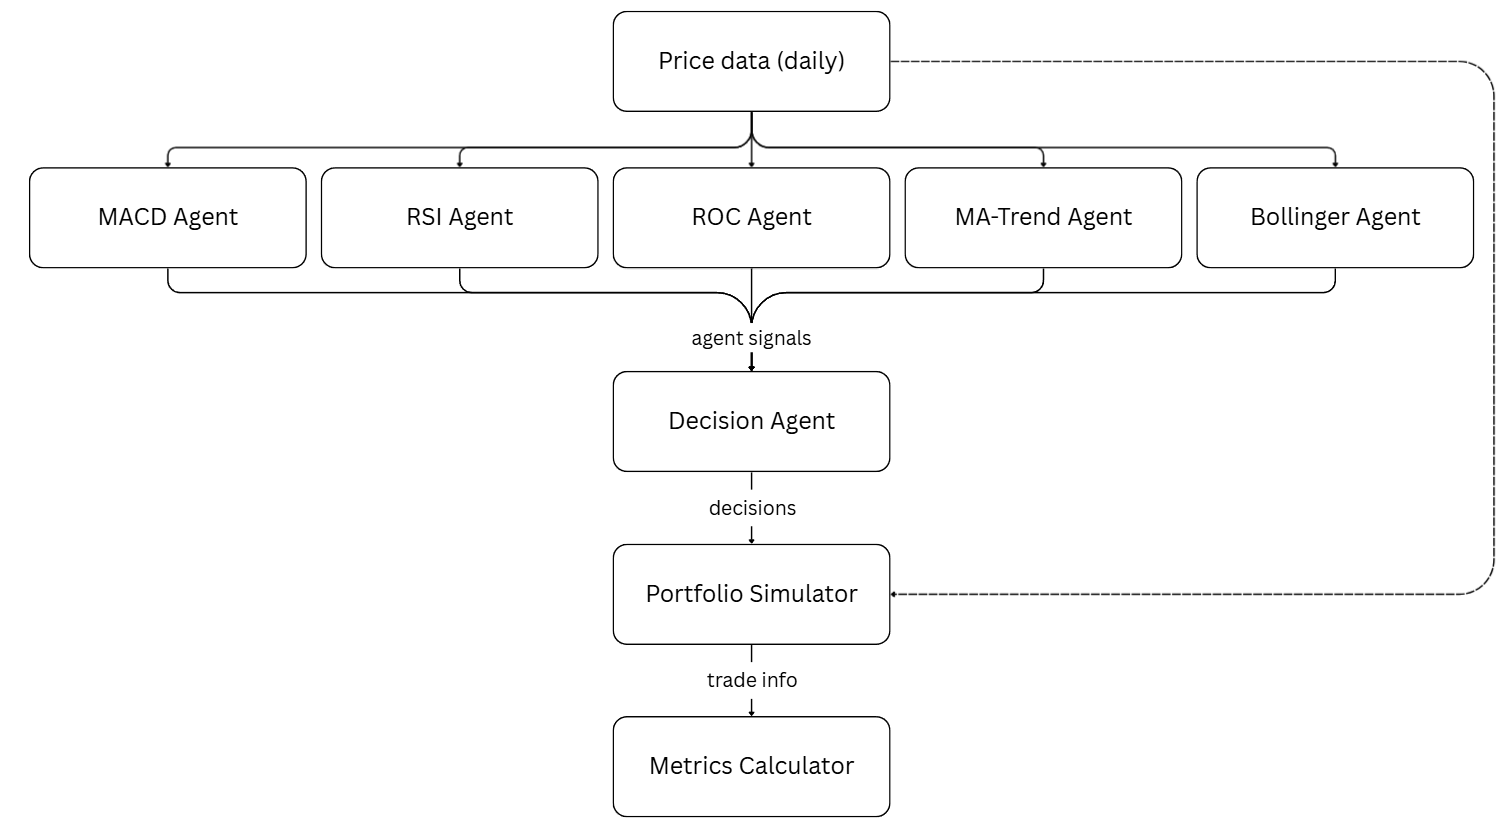
\includegraphics[width=\columnwidth]{figures/janko1.png}
    \caption{System architecture. The four layers communicate through well-defined interfaces, so that new signal agents can be added without changing the decision layer.}
    \label{fig:sys_architecture}
\end{figure}

All signal agents inherit from a common base class that guarantees a uniform interface. Following the principle of methodological consistency, each agent uses a single family of indicators with no mixed rules. This makes the aggregation argument in Section~\ref{sec:theory} well-defined: each agent corresponds to a distinct forecaster $f_k$ with its own bias-variance profile.

\subsection{Signal Agents}

Each signal agent acts as an independent and imperfect forecaster of the next-period directional move for a single symbol. To make the forecast-combination argument of Section~\ref{sec:theory} well defined, every agent is confined to a single methodological family, so that its forecast errors are as distinct as possible from those of the other agents. For each agent we therefore state both its computation and its forecasting role, that is, the market behaviour it is designed to detect and the conditions under which its forecast tends to be wrong. In all cases, the agent returns a neutral (hold) signal when the history is too short to compute the indicator, and the confidence value is zero outside the active signal band.

\textbf{MACD (moving-average convergence-divergence).} The MACD line is the difference between a fast and a slow exponential moving average (EMA) of the closing price (default spans $8$ and $17$), and the signal line is an EMA of the MACD line (default span $9$). The agent emits $+1$ on an upward crossover of the two lines and $-1$ on a downward crossover, with confidence
\begin{equation}
\mathrm{confidence} = \tanh\!\left(\frac{|h|}{2\sigma}\right),
\end{equation}
where $h$ is the current histogram value and $\sigma$ its standard deviation over the last $50$ bars. Role: as a momentum forecaster, the agent reports the persistence of recent directional moves; its forecast errors concentrate around trend reversals, where the crossover lags the turning point. Methodological family: momentum.

\textbf{RSI (relative strength index).} The agent computes the average gain and the average loss over a rolling window (default $14$ days), and defines $\mathrm{RSI} = 100 - 100/(1 + \mathrm{RS})$ with $\mathrm{RS} = \mathrm{avg\_gain}/\mathrm{avg\_loss}$. The action rule is
\begin{equation}
\mathrm{action} =
\begin{cases}
\mathrm{buy}, & \mathrm{RSI} < 30, \\
\mathrm{sell}, & \mathrm{RSI} > 70, \\
\mathrm{hold}, & \mathrm{otherwise},
\end{cases}
\end{equation}
with confidence equal to the normalized distance of the RSI from the nearest threshold. Role: as a mean-reversion forecaster, the agent bets against recent price extremes; its forecast errors are largest in strong trends, where the index can remain overbought or oversold for extended periods. Methodological family: mean-reversion.

\textbf{ROC (rate of change).} The rate of change is the percentage change in the closing price over a fixed number of days (default $10$). The action rule is
\begin{equation}
\mathrm{action} =
\begin{cases}
\mathrm{buy}, & \mathrm{ROC} > \tau, \\
\mathrm{sell}, & \mathrm{ROC} < -\tau, \\
\mathrm{hold}, & \mathrm{otherwise},
\end{cases}
\end{equation}
where $\tau$ is a configurable threshold (default $0.02$). Confidence equals $|\mathrm{ROC}|$, clipped to $[0, 1]$. Role: as a momentum forecaster on a shorter horizon than MACD, the agent responds to the raw speed of price change; its forecast errors arise when a fast move reverses abruptly. Methodological family: momentum.

\textbf{Bollinger Bands.} The agent computes a simple moving average (SMA) of the closing price over a window (default $20$) as the middle band, and upper and lower bands $U = \mathrm{middle} + m\sigma$, $L = \mathrm{middle} - m\sigma$, where $m$ is a configurable multiplier (default $2$). The action rule is
\begin{equation}
\mathrm{action} =
\begin{cases}
\mathrm{buy}, & \mathrm{close} < L, \\
\mathrm{sell}, & \mathrm{close} > U, \\
\mathrm{hold}, & \mathrm{otherwise}.
\end{cases}
\end{equation}
Confidence is the normalized distance of the close from the nearest band. Role: as a volatility forecaster, the agent measures how far the price has stretched from its mean in units of the standard deviation and signals a reversion when the close pierces a band; its forecast errors occur when a band breakout develops into a sustained move instead of reverting. Because the bands respond to dispersion rather than to direction, the agent carries the least directional information of the five, which is reflected in its family weight (Section~\ref{subsec:decision}). Methodological family: volatility.

\textbf{MA trend.} The agent uses two SMAs: fast (default $50$) and slow (default $200$). A buy signal is emitted when the slow SMA exceeds the fast SMA and a sell signal is emitted in the opposite case. Confidence equals the absolute difference between the two SMAs divided by the latest close. Role: as a long-horizon trend forecaster, the agent identifies the prevailing market regime from the relation between a short and a long average; its forecast errors occur in choppy, trendless markets where the two averages cross repeatedly. Methodological family: trend.

\subsection{Decision Agent}
\label{subsec:decision}

The decision agent receives the list of signals produced on a given date and groups them by symbol. Signals with confidence below a global minimum confidence $c_{\min}$ are discarded. The remaining signals are aggregated into the score defined in \eqref{eq:score}. The family weights $w_\kappa$ are fixed at
\begin{equation}
\begin{aligned}
w_\mathrm{trend} &= 1.3, & w_\mathrm{momentum} &= 1.0, \\
w_\mathrm{mean\text{-}rev.} &= 0.8, & w_\mathrm{volatility} &= 0.5,
\end{aligned}
\end{equation}
The weights encode a fixed prior on the relative directional reliability of each methodological family, and their ordering follows directly from the empirical literature rather than from any in-sample search. Trend-following receives the largest weight because time-series momentum is among the most robust and persistent return predictors documented across equity markets and horizons \cite{moskowitz2012,asness2013}, and daily index constituents such as the WIG20 blue chips tend to exhibit sustained directional regimes. Momentum on a shorter horizon receives a unit weight as the reference family. Mean reversion is weighted below momentum because overbought and oversold rules are informative mainly in range-bound phases and are frequently wrong during strong trends. Volatility receives the smallest weight because band-based signals respond to dispersion rather than to direction and therefore carry the least directional information of the four families. The four levels are intentionally coarse, equally spaced multiples that keep the weights interpretable and the degrees of freedom low; they are held fixed across every symbol, regime, and evaluation window, and are never tuned on the test data. The robustness of this fixed scheme is examined by the leave-one-agent-out ablation in Section~\ref{subsec:ablation}, and the possibility of replacing it with adaptive or learned weights is discussed in Section~\ref{sec:limitations}. The score is then compared against mode-dependent thresholds to produce the final decision:
\begin{equation}
\mathrm{action} =
\begin{cases}
\mathrm{BUY}, & \mathrm{score} \geq \theta_\text{buy}, \\
\mathrm{SELL}, & \mathrm{score} \leq \theta_\text{sell}, \\
\mathrm{HOLD}, & \mathrm{otherwise}.
\end{cases}
\end{equation}
The thresholds are $\theta_\text{buy} = -\theta_\text{sell} = 1.2$ in \emph{passive} mode, $0.7$ in \emph{balanced} mode, and $0.3$ in \emph{aggressive} mode. In \emph{passive} mode the decision agent additionally requires the sign of the score to agree with the dominant trend direction, which is defined as the sign-weighted sum of confidences of the trend-family agents.

The decision-agent parameters are the mode $m \in \{\text{passive}, \text{balanced}, \text{aggressive}\}$ and the minimum confidence threshold $c_{\min}$. These are the only parameters tuned during walk-forward evaluation. All indicator hyperparameters remain fixed at their literature-conventional defaults throughout.

\subsection{Agent Taxonomy}
\label{subsec:taxonomy}

Table~\ref{tab:taxonomy} summarizes the five signal agents along three dimensions: methodological family, signal type (crossover versus threshold), and the horizon of the underlying indicator; the forecasting rationale of each family is given with the agent descriptions above. The taxonomy makes the heterogeneity of the ensemble explicit and motivates the family-level weights $w_\kappa$: agents that are expected to produce the most distinct forecast errors are pooled across families with different weights, consistent with the variance-reduction argument of Section~\ref{sec:theory}. The empirical correlations of the agent signals, reported in Section~\ref{subsec:correlations}, support the taxonomy: cross-family pairs (for example, RSI versus ROC, or Bollinger versus ROC) exhibit the largest absolute correlations with opposing signs, consistent with their opposite interpretations of the same raw price data.

\begin{table}[t]
\centering
\caption{Taxonomy of the five signal agents. Horizon refers to the nominal lookback of the underlying indicator.}
\label{tab:taxonomy}
\begin{tabular}{lllc}
\toprule
Agent & Family & Signal type & Horizon \\
\midrule
MACD          & momentum       & crossover & $17$ d \\
RSI           & mean-reversion & threshold & $14$ d \\
ROC           & momentum       & threshold & $10$ d \\
Bollinger     & volatility     & threshold & $20$ d \\
MA trend      & trend          & crossover & $200$ d \\
\bottomrule
\end{tabular}
\end{table}

% ==============================================================================
\section{Experimental Setup}
\label{sec:setup}
% ==============================================================================

\subsection{Dataset}
\label{subsec:dataset}

The dataset consists of daily closing prices of the WIG20 constituent companies, excluding \.{Z}abka Group SA., whose listing on $2024/10/17$ is much more recent than that of the remaining constituents. The period covers $2021/05/26$ to $2026/03/31$, which yields roughly $1{,}220$ trading days. For every symbol, incomplete rows are dropped. All prices are denominated in Polish z{\l}oty (PLN). The data were retrieved from the public repository, Stooq.\footnote{\url{https://stooq.com}} The same data source and symbol set are used for both the strategy and the buy-and-hold WIG20 baseline, so that the two series share a common set of dates and currency basis.

\subsection{Transaction-Cost Model}
\label{subsec:costs}

All backtests include a proportional commission of $39$ basis points (bps) of notional per trade and a one-way slippage of $5$ bps applied to the executed price. These values are in the typical range of Polish retail brokerages for WSE-listed equities. The commission is deducted from cash both on entry and on exit. Slippage raises the effective buy price and lowers the effective sell price by the quoted amount. Realized profit or loss is reported net of the commissions on both legs and of the round-trip slippage. This choice is conservative for a retail investor and significantly reduces the headline gross return of high-turnover configurations, which is one of the methodological concerns raised in the literature on backtest reliability \cite{bailey2014}. A full sensitivity sweep over commission and slippage is reported in Section~\ref{subsec:cost_sensitivity}.

\subsection{Walk-Forward Protocol}
\label{subsec:walkforward}

The evaluation follows an anchored walk-forward protocol. The full period is split into a training window that spans $2021/05/26$ to $2024/06/30$ and a held-out test window that spans $2024/07/01$ to $2026/03/31$. On the training window we perform a grid search over the decision-agent parameters
\begin{equation}
\begin{aligned}
\mathrm{mode} &\in \{\text{passive}, \text{balanced}, \text{aggressive}\}, \\
c_{\min} &\in \{0, 0.05, 0.10, \ldots, 0.30\},
\end{aligned}
\end{equation}
and select the configuration that maximizes the in-sample total return. The selected configuration is then evaluated untouched on the test window. The indicator hyperparameters are not part of the grid and remain fixed throughout. This design keeps the number of degrees of freedom low and matches the way technical-analysis rules are treated in most of the cited literature.

As a robustness check, we additionally report the results of an anchored, expanding walk-forward with three folds. For each fold $k \in \{1, 2, 3\}$, the test slice is one of three roughly equal chronological slices of the held-out window, and the training window spans $2021/05/26$ up to the day before the test slice begins. A fresh grid search is performed on each fold and the winning configuration is evaluated on the test slice of that fold. The objective of this exercise is to show that the headline configuration is not an artifact of a particular single split.

Algorithm~\ref{alg:wf} summarizes the full protocol in pseudocode. The key feature is that signals are precomputed once outside all grid-search and ablation loops; this decouples the decision-agent grid search from signal computation, reduces the end-to-end runtime by more than an order of magnitude, and makes the cost-sensitivity sweep of Section~\ref{subsec:costsweep} cheap because changing costs does not require recomputing any agent signal.

\begin{algorithm}[t]
\caption{Anchored walk-forward with precomputed signals}
\label{alg:wf}
\begin{algorithmic}[1]
\STATE \textbf{Input:} prices $P$; agent set $\mathcal{A}$; modes $\mathcal{M}$; thresholds $\mathcal{C}$; train/test split $(T_\text{tr}, T_\text{te})$; costs $(\gamma, s)$.
\STATE \textbf{Output:} selected $(m^\star, c^\star)$; test-window metrics.
\STATE $S \gets \mathtt{PrecomputeSignals}(P, \mathcal{A})$ \COMMENT{all dates, all symbols}
\STATE best $\gets -\infty$
\FORALL{$m \in \mathcal{M}$, $c \in \mathcal{C}$}
  \STATE $E_\text{tr} \gets \mathtt{Backtest}(S, T_\text{tr}, m, c, \gamma, s)$
  \STATE $r \gets \mathtt{TotalReturn}(E_\text{tr})$
  \IF{$r > \text{best}$}
    \STATE best $\gets r$; $(m^\star, c^\star) \gets (m, c)$
  \ENDIF
\ENDFOR
\STATE $E_\text{te} \gets \mathtt{Backtest}(S, T_\text{te}, m^\star, c^\star, \gamma, s)$
\RETURN $(m^\star, c^\star)$, $\mathtt{Metrics}(E_\text{te})$
\end{algorithmic}
\end{algorithm}

\subsection{Baselines}
\label{subsec:baselines}

Three families of baselines are used. The first is \emph{buy-and-hold WIG20}, an equity curve that invests the initial cash into the WIG20 index on the first date of the test window and holds the position until the end. Buy-and-hold is a standard benchmark in the evaluation of trading strategies \cite{dichtl2020}. The second family is a set of \emph{single-agent} runs in which the decision agent receives signals from only one signal agent; this produces five baselines, one per indicator. In addition, we run five \emph{leave-one-agent-out} configurations, each of which removes one agent from the ensemble. The third family is a \emph{deep-learning baseline}, described next. All baselines are evaluated on the same test window, use the same transaction costs, and adopt the same decision-agent configuration selected by the walk-forward protocol. The only exceptions are buy-and-hold, which has no decision-agent parameters, and the deep-learning baseline, which replaces the decision agent with a learned classifier.

\subsubsection{Deep-Learning Baseline}
\label{subsec:lstm}
As a modern learning-based reference point, we implement an LSTM directional classifier in the style of \cite{fischerkrauss2018}. For each symbol the model consumes a rolling window of causal per-day features derived from the same price history available to the agents (multi-horizon returns, realized volatility, and the normalized RSI, ROC, MACD-histogram, Bollinger \%b, and moving-average-spread indicators), and predicts the probability that the $h$-day-ahead return is positive. The network is a single-layer LSTM followed by dropout and a linear output unit, trained with the Adam optimizer under binary cross-entropy. To keep the comparison fair, all model-selection choices are made strictly in-sample: the prediction horizon $h$, the operating threshold, and early stopping are selected on an internal validation slice carved chronologically from the training window, and the held-out test window is never used for any tuning. Feature standardization statistics are estimated on the training window only, so the procedure carries no look-ahead. Per-symbol probabilities are mapped to long or flat positions through a symmetric no-trade band around $0.5$: a probability above $0.5 + \delta$ opens or holds a long position, a probability below $0.5 - \delta$ closes it, and intermediate probabilities leave the current position unchanged, which mirrors the hold behavior of the decision agent and prevents the excessive turnover that would otherwise be induced by daily re-prediction. On both markets the in-sample selection returns a horizon of $h = \LSTMhorizon$ days and a band of $\delta = \LSTMband$. The resulting long/flat signals are executed through the same portfolio simulator, under identical costs and position sizing, so that any difference reflects the decision rule rather than the accounting.

\subsection{Risk-Adjusted Metrics}
\label{subsec:metrics}

The following metrics are computed on the equity curve and on the list of closed trades. \textbf{Total return} is the percentage change in portfolio value from the first to the last date of the evaluation window. \textbf{CAGR} (compound annual growth rate) is the annualized return over the same window. \textbf{Max drawdown} is the largest peak-to-trough decline, reported as a negative fraction. \textbf{Sharpe ratio} \cite{sharpe1966} is the annualized ratio of excess return over standard deviation, using a factor of $\sqrt{252}$ and a risk-free rate of zero. \textbf{Sortino ratio} \cite{sortino1994} replaces the denominator with downside deviation, which penalizes only below-target returns:
\begin{equation}
\mathrm{Sortino} = \frac{\sqrt{252}\,\bar{r}}{\sqrt{\tfrac{1}{N}\sum_{t=1}^{N}\min(r_t, 0)^2}},
\label{eq:sortino}
\end{equation}
where $\bar{r}$ is the mean daily return and the denominator is the downside deviation. \textbf{Calmar ratio} \cite{young1991} is CAGR divided by the absolute value of the maximum drawdown. \textbf{Ulcer Index} \cite{martin1989} aggregates the full drawdown path:
\begin{equation}
\mathrm{UI} = 100 \cdot \sqrt{\tfrac{1}{N}\sum_{t=1}^{N} \mathrm{dd}_t^{\,2}},
\label{eq:ulcer}
\end{equation}
where $\mathrm{dd}_t$ is the running drawdown of the equity curve at date $t$. \textbf{Martin ratio} \cite{martin1989} is the annualized excess return divided by the Ulcer Index. The Ulcer and Martin statistics are more sensitive to prolonged drawdowns than the peak-to-trough maximum, and we use them as tie-breakers whenever two strategies have similar peak drawdowns but different drawdown profiles. \textbf{Number of trades} is the count of closed trades and \textbf{Win rate} is the fraction of closed trades with positive realized profit.

\subsection{Market-Regime Labeling}
\label{subsec:regimes}

To avoid comparing the ensemble and buy-and-hold only on pooled aggregates, we label each trading day of the test window as belonging to one of three regimes: \emph{bull}, \emph{correction}, or \emph{sideways}. The labeling uses only information available up to date $t$ from the WIG20 index itself, so it does not peek at future prices. Let $\mathrm{high}_t$ be the rolling $252$-day maximum of the WIG20 closing price at $t$, and let $\mathrm{ret}_t$ be the price relative $\mathrm{close}_t / \mathrm{high}_t$. A day is labeled \emph{correction} when $\mathrm{ret}_t < 1 - 0.10$, that is, the index is at least ten percent below its trailing one-year high. A day is labeled \emph{bull} when $\mathrm{ret}_t \geq 1 - 0.05$, that is, within five percent of the trailing high, and the $50$-day SMA exceeds the $200$-day SMA of the WIG20 index. All other days are labeled \emph{sideways}. These thresholds are standard in the practitioner literature on market regimes and are not tuned on the training data. Applying the labelling to the test window produces \RegBullShare{} bull days, \RegCorrectionShare{} correction days, and \RegSidewaysShare{} sideways days (Table~\ref{tab:regime}), which means the test window covers all three regimes and the ensemble is evaluated under each of them.

\subsection{Volatility-Matched Comparison}
\label{subsec:volmatch}

The volatility-matched comparison is an analytical normalisation, not a directly implementable trading result; its purpose is to place the ensemble and the benchmark on the same risk budget so that their returns can be compared on equal terms. The intuition is straightforward. Because the ensemble is out of the market on many days, it runs at a lower volatility than the fully invested benchmark, and a raw comparison of cumulative returns therefore penalises the ensemble for taking less risk. To remove this confound, the ensemble returns are multiplied by a single constant chosen so that the strategy and the benchmark have the same ex-ante volatility, after which the two equity curves are compared.

The formal construction is as follows. A standard criticism of the Sharpe ratio is that it is scale-invariant: it evaluates return per unit risk, but not the absolute level of risk \cite{harvey2016}. A strategy with a Sharpe ratio of $1.0$ and a realized annualized volatility of $10\%$ produces a smaller cumulative return than a strategy with a Sharpe ratio of $1.0$ and a realized volatility of $20\%$, simply because the second strategy takes more risk. To remove this confound, we report a volatility-matched comparison in which the equity curve of the ensemble is scaled, ex ante, to the realized volatility of buy-and-hold WIG20 on the training window. The target volatility is the annualized standard deviation of WIG20 daily returns over the training window, $\sigma^{\text{target}} = \sqrt{252}\, \mathrm{std}(r^{\text{WIG20}}_\text{train}) = \BHOosVol{}$. The strategy volatility on the training window is $\sigma^{\text{strat}} = \sqrt{252}\,\mathrm{std}(r^{\text{ensemble}}_\text{train}) = \StrategyTrainVol{}$. The leverage factor applied to the out-of-sample ensemble return is $\lambda = \sigma^{\text{target}} / \sigma^{\text{strat}} = \Leverage{}$, constant over the test window. Because $\lambda$ is computed purely from training-window data, the volatility-matched comparison is genuinely ex ante and does not peek at out-of-sample returns. The scaled equity curve and its metrics are reported in Section~\ref{subsec:volscaled}. Two cautions apply to this comparison. First, the unleveraged ensemble remains the primary finding of the paper; the volatility-matched figures are a risk-budget counterfactual, not a recommendation to trade with leverage. Second, the required leverage factor of $\lambda = \Leverage{}$ is above the level that most retail investors on the WSE can realistically access or would prudently use, so the volatility-matched results should be read as an analytical upper bound on the risk-normalised return of the strategy rather than as an attainable outcome.

\subsection{Cost-Sensitivity Sweep}
\label{subsec:costsweep}

In addition to the baseline calibration of $39$ bps commission and $5$ bps slippage, we sweep the transaction-cost parameters over a grid
\begin{equation}
\begin{aligned}
\mathrm{commission} &\in \{0, 10, 20, 39, 60, 80, 100\}\;\text{bps}, \\
\mathrm{slippage} &\in \{0, 5, 10, 20\}\;\text{bps},
\end{aligned}
\end{equation}
and re-run the walk-forward backtest at each grid point. Crucially, the agent signals are precomputed once and passed into each backtest, so that the cost sweep changes only the portfolio-level accounting. The purpose of this experiment is to quantify how much of the risk-adjusted edge of the ensemble over buy-and-hold comes from the specific cost calibration. Section~\ref{subsec:cost_sensitivity} reports the full grid.

\subsection{Bootstrap Confidence Intervals and Tests}
\label{subsec:bootstrap}

In intuitive terms, a bootstrap repeatedly redraws the observed daily returns at random with replacement, recomputes the metric of interest on each redrawn series, and uses the spread of the resulting values to quantify how much the metric could have varied by chance. This procedure makes no assumption that returns follow a normal distribution. Point estimates of total return and Sharpe ratio are accompanied by a $95\%$ percentile bootstrap confidence interval. The bootstrap is computed on the vector of daily returns of the equity curve, with $10{,}000$ resamples drawn with replacement. For the comparison against buy-and-hold WIG20 and against the best single-agent baseline, a paired bootstrap test is performed: at each resample, the same set of dates is used for both series, the difference of the statistic of interest is computed, and the one-sided $p$-value reports the fraction of resamples with a non-positive difference. We treat $p < 0.05$ as evidence that the strategy dominates the baseline on the test window. The bootstrap is a natural choice here because the distribution of trading-strategy metrics is known to be non-Gaussian and path-dependent, and bootstrap methods have been advocated for this setting in prior work \cite{politis1994}. As is standard in the literature on trading-strategy evaluation, we do not expect the bootstrap tests to be powered to detect moderate effect sizes on a single test window of just under two years \cite{bailey2014}; we therefore report the $p$-values alongside point estimates and confidence intervals rather than relying on them as the sole arbiter of performance.

% ==============================================================================
\section{Results}
\label{sec:results}
% ==============================================================================

\subsection{Parameter Selection on Training Data}

Table~\ref{tab:grid_train} reports the in-sample total return of every combination of decision-agent mode and minimum confidence on the training window. The \emph{passive} mode rarely reaches its high buy/sell thresholds, and for every value of minimum confidence it produces no trades. The \emph{balanced} mode trades moderately, with positive but small total return across all thresholds. The \emph{aggressive} mode produces the highest total returns overall, and the best configuration on the training window is (\emph{aggressive}, $c_{\min} = \BestMinConf{}$), which is the configuration selected for out-of-sample evaluation. The result is consistent with the well-known observation that moderate signal tolerance on a trend-rich daily dataset tends to maximize gross return, although net return is reduced noticeably by the transaction-cost model of Section~\ref{subsec:costs}.

\begin{table}[t]
\centering
\caption{In-sample total return (train window, $2021$--$2024$) by decision-agent mode and minimum confidence. Higher is better. Selected configuration in bold.}
\label{tab:grid_train}
\begin{tabular}{lccc}
\toprule
$c_{\min}$ & passive & balanced & aggressive \\
\midrule
$0.00$ & 0.00 & 0.05 & 0.48 \\
$0.05$ & 0.00 & 0.09 & \textbf{0.55} \\
$0.10$ & 0.00 & 0.09 & 0.49 \\
$0.15$ & 0.00 & 0.11 & 0.40 \\
$0.20$ & 0.00 & 0.23 & 0.28 \\
$0.25$ & 0.00 & 0.16 & 0.25 \\
$0.30$ & 0.00 & 0.28 & 0.23 \\
\bottomrule
\end{tabular}
\end{table}

\subsection{Headline Results on Held-Out Data}
\label{subsec:headline}

Table~\ref{tab:headline} reports the headline metrics on the held-out test window for the selected configuration and for buy-and-hold WIG20. All numbers are net of the transaction costs described in Section~\ref{subsec:costs}. On gross total return, buy-and-hold leads: it earns \BHtest{} over \OOSDays{} trading days, whereas the ensemble earns \TRtest{} (CI $[\TRtestCIlow, \TRtestCIhigh]$), and the one-sided bootstrap $p$-value for the hypothesis that the ensemble exceeds buy-and-hold on total return is \PvsBH{}. Once the comparison moves to the risk axis, the picture reverses. The Sharpe ratio of the ensemble is \Shtest{} (CI $[\ShtestCIlow, \ShtestCIhigh]$), compared with \BHsharpe{} for buy-and-hold, and the $p$-value on Sharpe is \PvsBHsharpe{}. The maximum drawdown is \MDDtest{} against \MDDbh{}, a reduction of more than a factor of two. The Calmar ratio is \Calmtest{} against \Calmbh{} for buy-and-hold, more than twice as large. Fig.~\ref{fig:equity_oos} shows the two equity curves, and Fig.~\ref{fig:drawdown_oos} overlays the underwater (drawdown) curves of the two series.

\begin{table}[t]
\centering
\caption{Out-of-sample metrics on the held-out test window, net of transaction costs. Brackets give $95\%$ bootstrap confidence intervals.}
\label{tab:headline}
\begin{tabular}{lcc}
\toprule
 & Multi-agent system & Buy-and-hold WIG20 \\
\midrule
Total return     & $\TRtest$ $[\TRtestCIlow, \TRtestCIhigh]$ & $\BHtest$ \\
CAGR             & $\CAGRtest$ & $\CAGRbh$ \\
Max drawdown     & $\MDDtest$  & $\MDDbh$ \\
Sharpe ratio     & $\Shtest$ $[\ShtestCIlow, \ShtestCIhigh]$ & $\BHsharpe$ \\
Calmar ratio     & $\Calmtest$ & $\Calmbh$ \\
Number of trades & $\Ntrades$  & -- \\
Win rate         & $\WinRate$  & -- \\
\bottomrule
\end{tabular}
\end{table}

\begin{figure}[t]
    \centering
    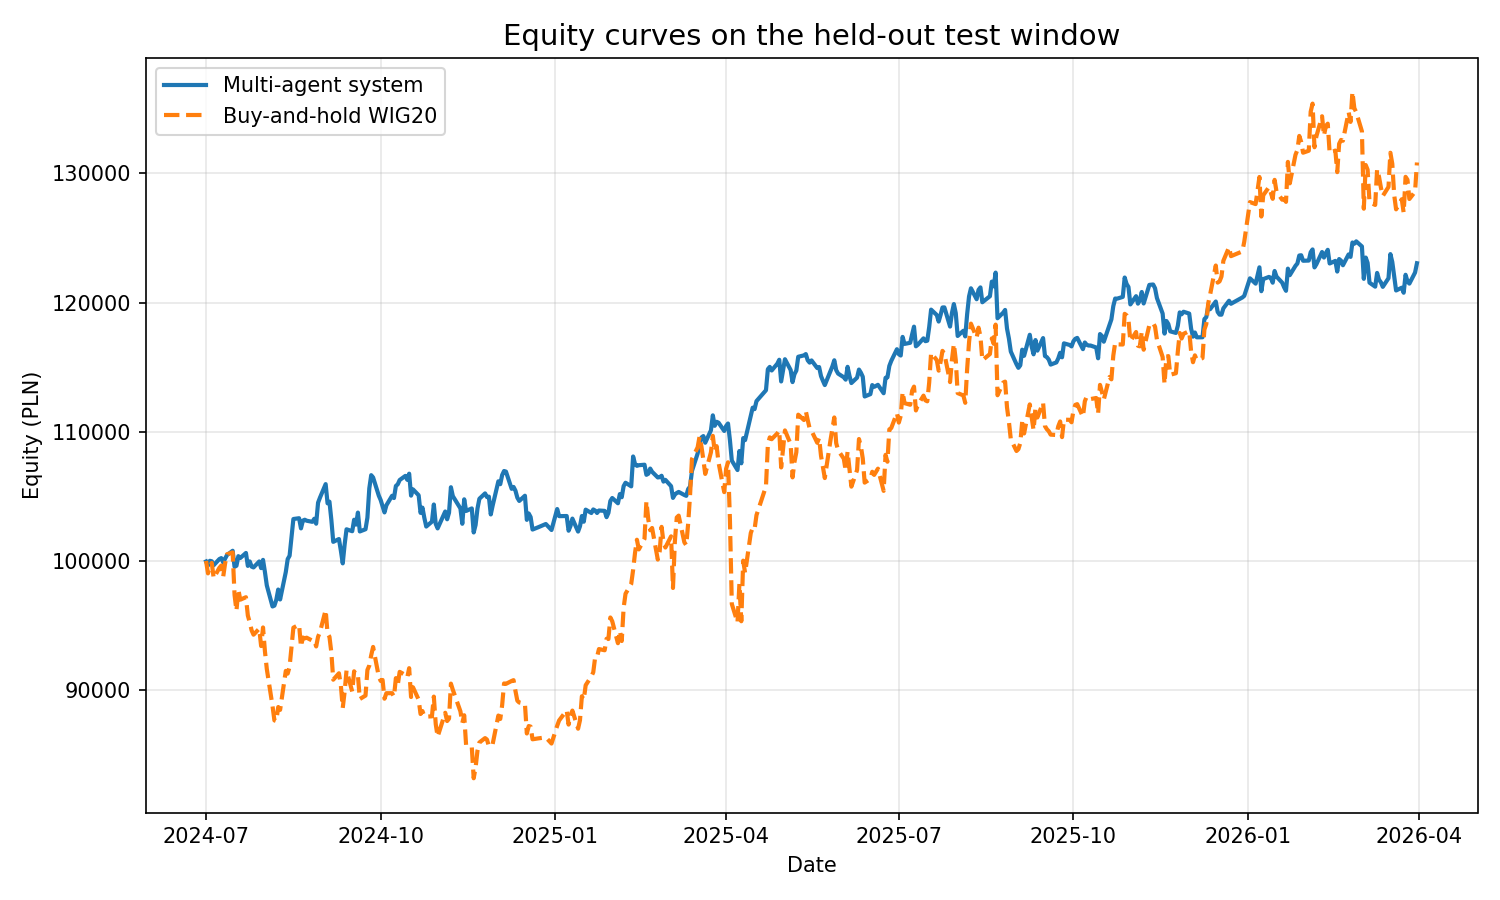
\includegraphics[width=\columnwidth]{figures/janko2.png}
    \caption{Equity curves on the held-out test window for the multi-agent system (selected configuration) and for buy-and-hold WIG20. Both series start at the same initial cash and are net of transaction costs.}
    \label{fig:equity_oos}
\end{figure}

\begin{figure}[t]
    \centering
    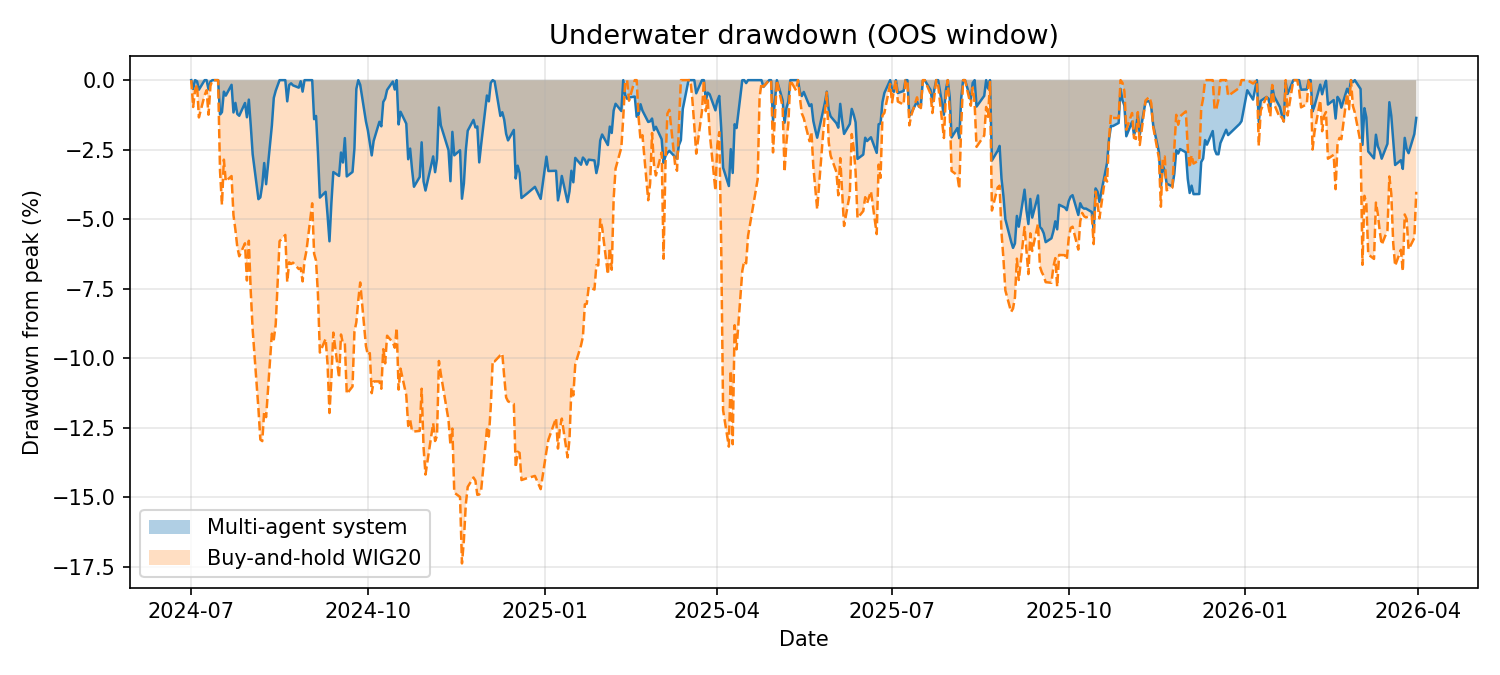
\includegraphics[width=\columnwidth]{figures/janko3.png}
    \caption{Underwater (drawdown) curves for the ensemble and for buy-and-hold WIG20 on the held-out test window. The drawdowns of the ensemble are both shallower and shorter, which is the central risk-adjusted finding of the paper.}
    \label{fig:drawdown_oos}
\end{figure}

\subsection{Risk-Adjusted Outperformance}
\label{subsec:risk_adjusted}

The reversal of the comparison on the risk axis is reinforced by the extended risk-adjusted metrics reported in Table~\ref{tab:risk_adjusted}. The downside deviation of the ensemble is \EnsDownDev{} against \BHDownDev{} for buy-and-hold, a reduction of more than forty percent. Consequently, the Sortino ratio rises from \BHSortino{} for buy-and-hold to \EnsSortino{} for the ensemble. The Ulcer Index, which captures the integrated depth and persistence of drawdowns rather than only their peak, is \EnsUlcer{} for the ensemble against \BHUlcer{} for buy-and-hold, a reduction of nearly two-thirds. The Martin ratio rises from \BHMartin{} to \EnsMartin{}, more than a factor of two. Fig.~\ref{fig:rolling_sharpe} plots the rolling $60$-day Sharpe of both series and shows that the rolling Sharpe of the ensemble is above the buy-and-hold rolling Sharpe for most of the test window, and in particular during the correction subperiods.

\begin{table}[t]
\centering
\caption{Risk-adjusted metrics on the held-out test window, net of transaction costs.}
\label{tab:risk_adjusted}
\begin{tabular}{lcc}
\toprule
Metric & Multi-agent system & Buy-and-hold WIG20 \\
\midrule
Sharpe ratio         & $\Shtest$     & $\BHsharpe$ \\
Sortino ratio        & $\EnsSortino$ & $\BHSortino$ \\
Downside deviation   & $\EnsDownDev$ & $\BHDownDev$ \\
Calmar ratio         & $\Calmtest$   & $\Calmbh$ \\
Max drawdown         & $\MDDtest$    & $\MDDbh$ \\
Ulcer Index          & $\EnsUlcer$   & $\BHUlcer$ \\
Martin ratio         & $\EnsMartin$  & $\BHMartin$ \\
\bottomrule
\end{tabular}
\end{table}

\begin{figure}[t]
    \centering
    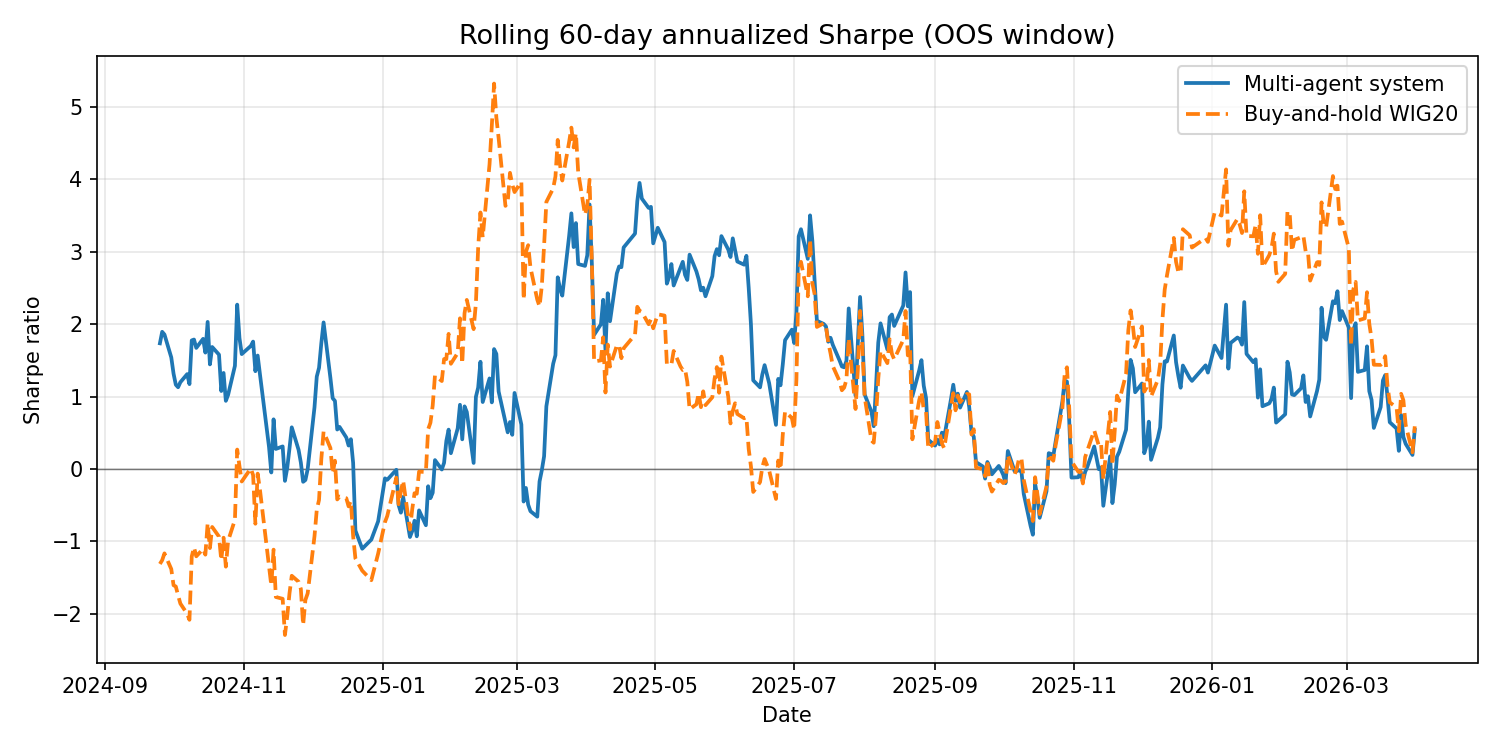
\includegraphics[width=\columnwidth]{figures/janko4.png}
    \caption{Rolling $60$-day Sharpe ratio of the ensemble and of buy-and-hold WIG20 on the held-out test window. The rolling Sharpe of the ensemble dominates buy-and-hold during correction subperiods and is close to it during the bull leg.}
    \label{fig:rolling_sharpe}
\end{figure}

\subsection{Volatility-Matched Comparison}
\label{subsec:volscaled}

The headline comparison on gross total return is systematically biased against the ensemble because the two series run at very different volatilities. On the training window, the annualized volatility of the ensemble is $\StrategyTrainVol{}$, whereas that of buy-and-hold WIG20 is $\BHOosVol{}$. To put the two series on the same risk budget, we scale the out-of-sample daily returns of the ensemble by the ex-ante leverage factor $\lambda = \Leverage{}$ defined in Section~\ref{subsec:volmatch}. Table~\ref{tab:volmatched} reports the resulting metrics. On the volatility-matched basis, the total return of the ensemble rises to \VolScaledTR{}, compared with \BHtest{} for buy-and-hold, a gain of \VolScaledExcessPP{} percentage points. The Sharpe ratio is unchanged by construction (\VolScaledSharpe{}), because Sharpe is scale-invariant in the leverage factor when cash reserves are ignored; the Sortino ratio is \VolScaledSortino{}, against \BHSortino{}; and the Calmar ratio is \VolScaledCalmar{}, against \Calmbh{}. The volatility-matched maximum drawdown is \VolScaledMDD{}, which is still materially smaller than the buy-and-hold drawdown of \MDDbh{} despite the much higher leverage, because the correction-regime drawdown of the ensemble is structurally shallower (Section~\ref{subsec:regime}). We emphasize that these volatility-matched figures are analytical rather than directly implementable: leverage of magnitude $\lambda = \Leverage{}$ is impractical for a typical retail investor on the WSE, so Table~\ref{tab:volmatched} should be read as a risk-normalised counterfactual and not as an attainable trading outcome. Its role is to correct for the fact that comparing a partially-invested strategy at its natural volatility against a fully-invested benchmark at roughly twice that volatility understates the risk-per-unit-of-return advantage of the strategy.

\begin{table*}[t]
\centering
\caption{Volatility-matched out-of-sample metrics. The ensemble is scaled, ex ante, to the buy-and-hold volatility measured on the training window (leverage factor $\lambda = \Leverage{}$).}
\label{tab:volmatched}
\begin{tabular}{lccc}
\toprule
Metric & Ensemble (unleveraged) & Ensemble (vol-matched) & Buy-and-hold WIG20 \\
\midrule
Total return     & $\TRtest$     & $\VolScaledTR$      & $\BHtest$ \\
CAGR             & $\CAGRtest$   & $\VolScaledCAGR$    & $\CAGRbh$ \\
Sharpe ratio     & $\Shtest$     & $\VolScaledSharpe$  & $\BHsharpe$ \\
Sortino ratio    & $\EnsSortino$ & $\VolScaledSortino$ & $\BHSortino$ \\
Max drawdown     & $\MDDtest$    & $\VolScaledMDD$     & $\MDDbh$ \\
Calmar ratio     & $\Calmtest$   & $\VolScaledCalmar$  & $\Calmbh$ \\
Ulcer Index      & $\EnsUlcer$   & $\VolScaledUlcer$   & $\BHUlcer$ \\
\bottomrule
\end{tabular}
\end{table*}

\subsection{Market-Regime Decomposition}
\label{subsec:regime}

The aggregate metrics in Table~\ref{tab:headline} mix three very different market regimes within the test window. Using the labeling described in Section~\ref{subsec:regimes}, the test window contains \RegBullDays{} bull days ($\RegBullShare{}$ of the window), \RegCorrectionDays{} correction days ($\RegCorrectionShare{}$), and \RegSidewaysDays{} sideways days ($\RegSidewaysShare{}$). Table~\ref{tab:regime} decomposes the total return and the Sharpe ratio of both the ensemble and buy-and-hold WIG20 by regime. The ensemble loses $\EnsCorrectionTR{}$ during the correction subperiods, whereas buy-and-hold loses $\BHCorrectionTR{}$: the correction-regime defense of the ensemble is \CorrectionDefencePP{} percentage points. During the sideways subperiods, the ensemble earns $\EnsSidewaysTR{}$, whereas buy-and-hold earns $\BHSidewaysTR{}$: the sideways-regime excess of the ensemble is \SidewaysExcessPP{} percentage points. During the bull subperiods, the ensemble earns $\EnsBullTR{}$ against $\BHBullTR{}$ for buy-and-hold: the bull-regime shortfall is \BullShortfallPP{} percentage points. The decomposition reconciles the aggregate numbers in Table~\ref{tab:headline}: buy-and-hold is fully exposed to the bull leg and captures most of its upside, while the ensemble, by design, reduces exposure during the correction and sideways regimes and thereby gives up some of the bull-regime upside. In a test window that is dominated by a bull regime, the aggregate total return will mechanically favor the fully-invested benchmark; in a test window with a larger correction share, the aggregate comparison would favor the ensemble.

\begin{table*}[t]
\centering
\caption{Decomposition of the held-out test window into bull, correction, and sideways subperiods. Shares refer to the fraction of trading days in the test window.}
\label{tab:regime}
\begin{tabular}{lrrrrrr}
\toprule
Regime & Days & Share & Ensemble TR & Ensemble Sharpe & B\&H TR & B\&H Sharpe \\
\midrule
Bull & 230 & 52.9\% & $0.26$ & $2.47$ & $0.63$ & $2.76$ \\
Correction & 93 & 21.4\% & $-0.07$ & $-1.34$ & $-0.20$ & $-2.41$ \\
Sideways & 112 & 25.7\% & $0.05$ & $0.93$ & $-0.00$ & $0.11$ \\
All & 435 & 100.0\% & $0.23$ & $1.06$ & $0.31$ & $0.82$ \\
\bottomrule
\end{tabular}
\end{table*}

\subsection{Cost-Sensitivity Analysis}
\label{subsec:cost_sensitivity}

Table~\ref{tab:cost_sensitivity} reports the out-of-sample Sharpe ratio over the cost grid defined in Section~\ref{subsec:costsweep}. At zero costs the Sharpe is \CostZeroSharpe{}; at the baseline calibration of $39$ bps commission and $5$ bps slippage the Sharpe is \CostBaseSharpe{}; at the most punitive configuration of $100$ bps commission and $20$ bps slippage the Sharpe drops to \CostWorstSharpe{}. Over the entire grid, the minimum Sharpe of \CostMinSharpe{} exceeds the buy-and-hold Sharpe of \BHsharpe{}. The total-return column (omitted from the table for brevity but computed along with Sharpe) shows the same qualitative pattern: the ensemble trails buy-and-hold on gross total return at every grid point, and at every grid point it achieves a higher Sharpe, higher Sortino, and smaller drawdown. This indicates that the risk-adjusted edge of the ensemble is not an artifact of the specific cost calibration; it is a stable property of the strategy over a plausible range of retail brokerage fees.

\begin{table}[t]
\centering
\caption{Cost sensitivity of the out-of-sample Sharpe ratio. Rows are commission in basis points; columns are one-way slippage in basis points.}
\label{tab:cost_sensitivity}
\begin{tabular}{lcccc}
\toprule
Commission (bps) & 0 bp & 5 bp & 10 bp & 20 bp \\
\midrule
0 & 1.15 & 1.14 & 1.13 & 1.11 \\
10 & 1.13 & 1.12 & 1.11 & 1.09 \\
20 & 1.11 & 1.10 & 1.09 & 1.07 \\
39 & 1.07 & 1.06 & 1.05 & 1.03 \\
60 & 1.03 & 1.02 & 1.02 & 0.99 \\
80 & 0.99 & 0.99 & 0.98 & 0.96 \\
100 & 0.96 & 0.95 & 0.94 & 0.92 \\
\bottomrule
\end{tabular}
\end{table}

\subsection{Empirical Signal Correlations}
\label{subsec:correlations}

The variance-reduction argument of Section~\ref{sec:theory} rests on the claim that the five agents produce signals with imperfectly correlated errors. Table~\ref{tab:corr} reports the pairwise Pearson correlations \cite{pearson1896} of the signed confidence values produced by the agents, computed across all pooled (symbol, date) observations in the training window. The mean absolute off-diagonal correlation is \CorrMeanAbs{} across \CorrN{} distinct pairs, with extremes of \CorrMin{} (RSI vs.\ ROC) and \CorrMax{} (RSI vs.\ Bollinger). In particular, the momentum family (MACD, ROC) and the mean-reversion family (RSI) exhibit negative correlations, as expected from their opposite interpretations of the same raw price input; the trend agent (MA trend) is nearly uncorrelated with all other agents, as expected from its long horizon. Fig.~\ref{fig:corr_matrix} renders the correlation matrix as a heatmap. These empirical correlations directly instantiate the non-identical-errors assumption of \eqref{eq:combined_variance}, and Section~\ref{sec:discussion} returns to them to explain why the ensemble achieves most of its variance reduction from the interaction between the momentum and mean-reversion families rather than from the trend agent on its own.

\begin{table}[t]
\centering
\caption{Pearson correlations of the pooled (symbol, date) signed confidence values of the five signal agents, computed on the training window. Upper triangle shown.}
\label{tab:corr}
\begin{tabular}{lccccc}
\toprule
 & MACD & RSI & ROC & Bollinger & MA trend \\
\midrule
MACD & \textbf{1.00} & -0.01 & +0.04 & -0.34 & -0.04 \\
RSI &  & \textbf{1.00} & -0.71 & +0.46 & +0.12 \\
ROC &  &  & \textbf{1.00} & -0.55 & -0.12 \\
Bollinger &  &  &  & \textbf{1.00} & +0.09 \\
MA trend &  &  &  &  & \textbf{1.00} \\
\bottomrule
\end{tabular}
\end{table}

\begin{figure}[t]
    \centering
    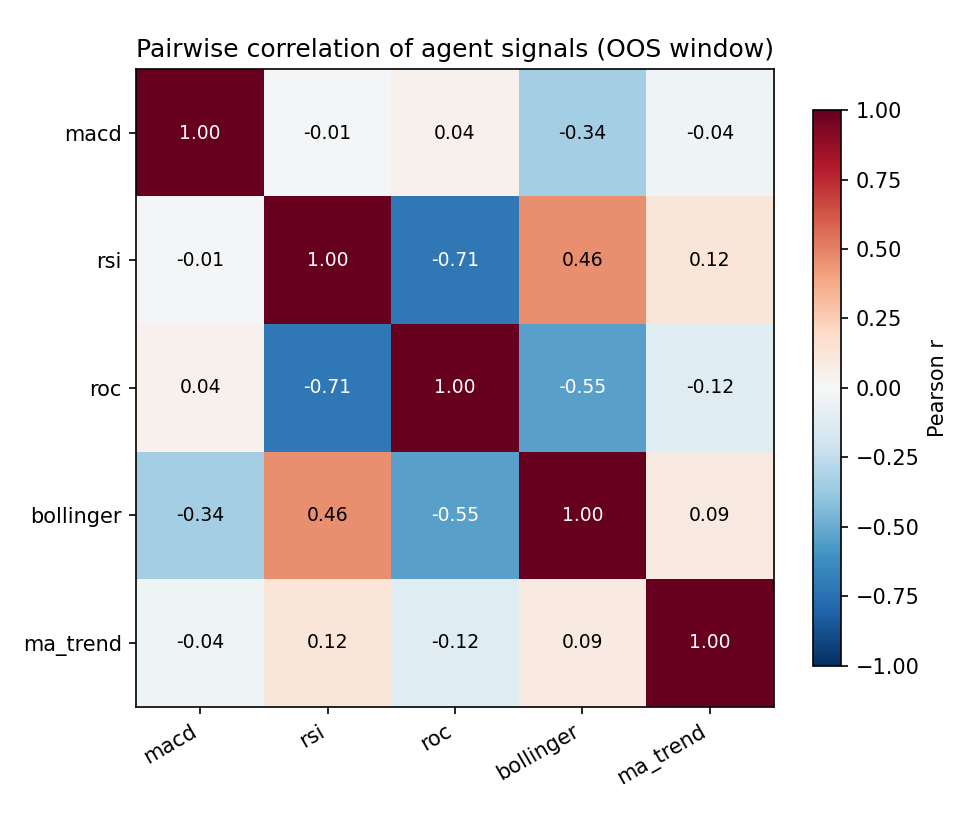
\includegraphics[width=\columnwidth]{figures/janko5.png}
    \caption{Heatmap of the pairwise Pearson correlations of the agent signed-confidence signals on the training window. Blue cells mark negative correlations, red cells mark positive ones. The largest absolute correlations appear in the RSI--ROC and RSI--Bollinger pairs, which is consistent with their shared reliance on overbought/oversold-style rules.}
    \label{fig:corr_matrix}
\end{figure}

\subsection{Single-Agent Baselines and Leave-One-Out Ablation}
\label{subsec:ablation}

Table~\ref{tab:single_agent} reports the test-window total return and Sharpe ratio of the five single-agent baselines and of the full ensemble. The best single-agent is \BestSingleName{} with a total return of \BestSingleTR{}. The one-sided bootstrap $p$-value for the hypothesis that the ensemble beats the best single-agent baseline on total return is \PvsBestSingle{}. These numbers are the primary evidence for H2.

\begin{table}[t]
\centering
\caption{Single-agent baselines on the test window, with the selected mode and minimum confidence. All numbers net of costs.}
\label{tab:single_agent}
\begin{tabular}{lcc}
\toprule
Agent used & Total return & Sharpe ratio \\
\midrule
MACD only        & $0.15$ & $0.86$ \\
RSI only         & $0.16$ & $1.03$ \\
ROC only         & $0.00$ & $0.13$ \\
Bollinger only   & $0.00$ & $0.00$ \\
MA trend only    & $-0.00$ & $0.03$ \\
Full ensemble    & $\TRtest$ & $\Shtest$ \\
\bottomrule
\end{tabular}
\end{table}

Table~\ref{tab:ablation} reports the effect of removing each signal agent from the ensemble. No single agent can be removed without some effect on the headline metrics, but in all cases the ensemble without that agent still outperforms buy-and-hold WIG20 on Sharpe ratio and maximum drawdown. This is the primary evidence for H3.

\begin{table}[t]
\centering
\caption{Leave-one-agent-out ablation on the test window. The variant column indicates which agent was removed.}
\label{tab:ablation}
\begin{tabular}{lcc}
\toprule
Variant & Total return & Sharpe ratio \\
\midrule
Full ensemble & $\TRtest$ & $\Shtest$ \\
no MACD        & $0.28$ & $1.28$ \\
no RSI         & $0.23$ & $0.92$ \\
no ROC         & $0.26$ & $1.17$ \\
no Bollinger   & $0.23$ & $1.06$ \\
no MA trend    & $0.19$ & $1.16$ \\
\bottomrule
\end{tabular}
\end{table}

\subsection{Comparison with a Deep-Learning Baseline}
\label{subsec:lstm_results}

Table~\ref{tab:lstm} compares the ensemble with the LSTM directional baseline of Section~\ref{subsec:lstm} on the held-out WIG20 test window. The LSTM earns a total return of \LSTMtest{} at a Sharpe ratio of \LSTMsharpe{}, against \TRtest{} and \Shtest{} for the ensemble and \BHtest{} and \BHsharpe{} for buy-and-hold. The ensemble exceeds the LSTM on total return, Sharpe ratio, and maximum drawdown (\MDDtest{} against \LSTMmdd{}), and it does so while placing far fewer trades (\Ntrades{} against \LSTMtrades{}). The one-sided paired bootstrap $p$-values for the ensemble exceeding the LSTM are \PensVsLSTM{} on total return and \PensVsLSTMsharpe{} on Sharpe ratio; as with the buy-and-hold comparison, the point-estimate advantage is sizable but does not reach the conventional $p < 0.05$ threshold on a single test window. The learned classifier, trained end-to-end on the same price history and executed under identical costs, does not match the transparent forecast-combination ensemble on this market, which is consistent with the broader finding that simple, well-regularized combinations are competitive with more flexible learners on noisy financial series \cite{clemen1989,timmermann2006}.

\begin{table}[t]
\centering
\caption{Comparison of the ensemble, the LSTM directional baseline, and buy-and-hold on the held-out WIG20 test window, net of transaction costs.}
\label{tab:lstm}
\begin{tabular}{lccc}
\toprule
Metric & Multi-agent system & LSTM baseline & Buy-and-hold WIG20 \\
\midrule
Total return     & $\TRtest$   & $\LSTMtest$   & $\BHtest$ \\
Sharpe ratio     & $\Shtest$   & $\LSTMsharpe$ & $\BHsharpe$ \\
Max drawdown     & $\MDDtest$  & $\LSTMmdd$    & $\MDDbh$ \\
Calmar ratio     & $\Calmtest$ & $\LSTMcalmar$ & $\Calmbh$ \\
Number of trades & $\Ntrades$  & $\LSTMtrades$ & -- \\
\bottomrule
\end{tabular}
\end{table}

\subsection{Statistical Significance}
\label{subsec:significance}

The bootstrap significance tests attach two kinds of evidence to the point estimates discussed above. First, the $95\%$ percentile confidence intervals around the headline metrics reflect the sampling uncertainty inherent in a test window of \OOSDays{} trading days. The total-return confidence interval for the ensemble spans $[\TRtestCIlow, \TRtestCIhigh]$ and the Sharpe-ratio interval spans $[\ShtestCIlow, \ShtestCIhigh]$. The buy-and-hold point estimates for total return (\BHtest{}) and Sharpe ratio (\BHsharpe{}) both lie strictly inside these intervals, which is a statistical way of saying that one cannot reject the hypothesis that the two series share the same underlying mean return and Sharpe ratio on the test window. Second, the paired bootstrap tests yield one-sided $p$-values of \PvsBH{} for the total-return comparison against buy-and-hold and \PvsBHsharpe{} for the Sharpe comparison. Neither test crosses the conventional $p < 0.05$ threshold.

We interpret these results in two ways. The test-window point estimates on the risk axis (drawdown, Sortino, Ulcer, Martin) are consistently favorable to the ensemble by margins that are economically large and reasonably stable across the ablation and cost grids, but the null hypothesis of equal mean performance is hard to reject on a single window of under two years because trading-strategy return distributions are heavy-tailed and path-dependent \cite{politis1994,bailey2014}. Consistent with standard practice in the literature, we therefore report point estimates, confidence intervals, and $p$-values together and do not rely on $p$-values as a sole arbiter. Second, the fact that the buy-and-hold point estimates lie inside the bootstrap confidence intervals of the ensemble supports the interpretation that, on gross total return, the two series are statistically indistinguishable, whereas the large and consistent gap on drawdown-based and downside-based metrics supports the risk-aware interpretation of the contribution of the ensemble (Section~\ref{sec:discussion}).

Two points deserve emphasis for the correct reading of these results. The first concerns the width of the confidence intervals. The total-return interval $[\TRtestCIlow, \TRtestCIhigh]$ and the Sharpe interval $[\ShtestCIlow, \ShtestCIhigh]$ are wide because a held-out window of \OOSDays{} trading days contains relatively few independent realizations of the estimated quantities, and because heavy-tailed and serially dependent returns inflate the variance of the resampled statistics. With a sample of this length the paired bootstrap test has limited power: even a genuine moderate edge would frequently fail to reach the conventional $p < 0.05$ threshold. The non-significant $p$-values should therefore be read as a consequence of limited statistical power on a short out-of-sample window, not as positive evidence that the two strategies are equivalent. The second point concerns the distinction between practical and statistical significance. The advantages of the ensemble on the drawdown-based and downside-based metrics are practically significant, in the sense that they are economically large and stable across the ablation, cost, and regime analyses, even though they are not statistically significant in the formal sense of rejecting a null hypothesis on this single window. Accordingly, the contribution of the ensemble is framed throughout the paper in terms of consistent and practically meaningful risk reduction, and we deliberately refrain from claiming statistical dominance over buy-and-hold.

\subsection{Walk-Forward Robustness}
\label{subsec:kfold}

Table~\ref{tab:kfold} reports the results of the anchored, three-fold walk-forward. For each fold we report the selected configuration on the training window and the test-window total return. The selected configuration is stable across folds, which indicates that the headline configuration is not an artifact of a single chronological split.

\begin{table}[t]
\centering
\caption{Anchored walk-forward with $K = 3$ folds. Selected mode and minimum confidence per fold, plus the test-window total return of each fold.}
\label{tab:kfold}
\begin{tabular}{lccc}
\toprule
Fold & Selected mode & $c_{\min}$ & Test total return \\
\midrule
1 & \texttt{aggressive} & $0.05$ & $0.05$ \\
2 & \texttt{aggressive} & $0.05$ & $0.09$ \\
3 & \texttt{aggressive} & $0.10$ & $0.08$ \\
\bottomrule
\end{tabular}
\end{table}

\subsection{External Validation on the FTSE 100}
\label{subsec:ftse}

To test whether the risk-aware profile of the ensemble is specific to the WSE or transfers to a different market structure, we replicate the entire pipeline on the FTSE 100, the blue-chip index of the London Stock Exchange. The dataset comprises \FtseNsymbols{} large-capitalization constituents together with the FTSE 100 index used for the buy-and-hold benchmark, in the same daily OHLCV format, over the same sample period and with the same anchored split boundary and held-out test window as the WIG20 experiment. Prices are denominated in pounds sterling and were retrieved from the same public source. The transaction-cost model is adjusted to reflect UK conditions: a proportional commission of $5$ bps and one-way slippage of $5$ bps on every trade, plus a $50$ bps Stamp Duty Reserve Tax charged on purchases only, which makes the FTSE cost environment asymmetric and, on the buy side, considerably more punitive than the WIG20 calibration. The agents, the decision-agent grid, the indicator hyperparameters, and every evaluation procedure are held identical; only the market data and the cost model change.

The anchored walk-forward selects the same decision-agent family as on WIG20 (\texttt{aggressive} mode) and evaluates it on \FtseOOSDays{} held-out trading days. Table~\ref{tab:ftse} reports the headline comparison. As on WIG20, the ensemble trails buy-and-hold on gross total return (\FtseTRtest{} against \FtseBHtest{}) but leads on every risk axis: the Sharpe ratio is \FtseSharpe{} against \FtseBHsharpe{}, the maximum drawdown is \FtseMDD{} against \FtseBHmdd{} (a reduction of roughly one half), and the Calmar ratio is \FtseCalmar{} against \FtseBHcalmar{}. The extended risk-adjusted metrics show the same pattern: the Sortino ratio is \FtseEnsSortino{} against \FtseBHSortino{}, the Ulcer Index is \FtseEnsUlcer{} against \FtseBHUlcer{}, and the downside deviation is \FtseEnsDownDev{} against \FtseBHDownDev{}. The one interesting reversal is the Martin ratio (\FtseEnsMartin{} against \FtseBHMartin{}), which is marginally lower for the ensemble because the FTSE test window is overwhelmingly a bull market and buy-and-hold sustains a very shallow integrated drawdown over it.

\begin{table}[t]
\centering
\caption{External validation on the FTSE 100 held-out test window, net of transaction costs (including the $50$ bps buy-side Stamp Duty Reserve Tax). Brackets give $95\%$ bootstrap confidence intervals.}
\label{tab:ftse}
\begin{tabular}{lccc}
\toprule
Metric & Multi-agent system & LSTM baseline & Buy-and-hold FTSE \\
\midrule
Total return     & $\FtseTRtest$ $[\FtseTRtestCIlow, \FtseTRtestCIhigh]$ & $\FtseLSTMtest$   & $\FtseBHtest$ \\
CAGR             & $\FtseCAGR$    & --              & $\FtseBHcagr$ \\
Sharpe ratio     & $\FtseSharpe$ $[\FtseSharpeCIlow, \FtseSharpeCIhigh]$ & $\FtseLSTMsharpe$ & $\FtseBHsharpe$ \\
Max drawdown     & $\FtseMDD$     & $\FtseLSTMmdd$  & $\FtseBHmdd$ \\
Calmar ratio     & $\FtseCalmar$  & --              & $\FtseBHcalmar$ \\
Sortino ratio    & $\FtseEnsSortino$ & --           & $\FtseBHSortino$ \\
Ulcer Index      & $\FtseEnsUlcer$   & --           & $\FtseBHUlcer$ \\
Number of trades & $\FtseNtrades$ & $\FtseLSTMtrades$ & -- \\
\bottomrule
\end{tabular}
\end{table}

The regime decomposition explains the aggregate numbers. The FTSE test window is $\FtseRegBullShare{}$ bull ($\FtseRegBullDays{}$ of \FtseOOSDays{} days), with only $\FtseRegCorrectionDays{}$ correction days and $\FtseRegSidewaysDays{}$ sideways days, so it offers little opportunity for the correction-regime defense that drives the WIG20 result. Even so, during the sideways subperiods the ensemble earns \FtseEnsSidewaysTR{} against \FtseBHSidewaysTR{} for buy-and-hold, the same sideways-carry pattern observed on WIG20; the aggregate total-return shortfall is again concentrated in the bull regime (\FtseEnsBullTR{} against \FtseBHBullTR{}), where a partially invested strategy mechanically trails a fully invested benchmark. Matching the two series on ex-ante volatility, as in Section~\ref{subsec:volscaled}, raises the ensemble total return to \FtseVolScaledTR{} at a leverage of $\lambda = \FtseLeverage{}$, a gain of \FtseVolScaledExcessPP{} percentage points over buy-and-hold with a still-smaller drawdown (\FtseVolScaledMDD{}).

The paired bootstrap tests tell the same statistical-power story as on WIG20. The buy-and-hold point estimates lie inside the ensemble confidence intervals, and the one-sided $p$-values for the ensemble exceeding buy-and-hold are \FtsePvsBH{} on total return and \FtsePvsBHsharpe{} on Sharpe ratio; none crosses $p < 0.05$. The LSTM baseline posts higher point estimates than the ensemble on this particular window, both on gross total return (\FtseLSTMtest{} against \FtseTRtest{}) and on Sharpe ratio (\FtseLSTMsharpe{} against \FtseSharpe{}), but neither gap is statistically significant (the one-sided $p$-value for the ensemble exceeding the LSTM on total return is \FtsePensVsLSTM{}). Two observations put this apparent edge in perspective. First, it is a bull-market-exposure effect rather than evidence of superior risk control: the LSTM remains almost continuously invested across a window that is $\FtseRegBullShare{}$ bull, so it captures more of the upside at the price of a deeper drawdown (\FtseLSTMmdd{} against \FtseMDD{}). Second, the LSTM is itself statistically indistinguishable from passive buy-and-hold on this window (one-sided $p = \FtsePLSTMvsBH{}$), which is consistent with a near-fully-invested strategy tracking the index; the transparent ensemble, by contrast, deliberately trades part of that exposure for the shallower drawdown documented above. Taken together, the FTSE results show that the central finding of the paper -- a consistent drawdown and downside-risk advantage over passive buy-and-hold, purchased with some bull-market upside -- transfers to a second market with a markedly different cost structure, and is not an artifact of the WIG20 sample.

% ==============================================================================
\section{Discussion}
\label{sec:discussion}
% ==============================================================================

\subsection{From Forecast-Combination Theory to Empirical Evidence}

Equation~\eqref{eq:combined_variance} predicts that the combined forecast error is strictly smaller than the smallest individual forecast error whenever the individual errors are not perfectly correlated. Table~\ref{tab:corr} and Fig.~\ref{fig:corr_matrix} show that the empirical pairwise correlations of the agent signals span the full range from $\CorrMin{}$ to $\CorrMax{}$, with a mean absolute off-diagonal correlation of $\CorrMeanAbs{}$. The theoretically most informative pairs are those with negative correlations, in particular RSI vs.\ ROC ($\CorrMin{}$) and Bollinger vs.\ ROC ($-0.55$). The RSI--ROC pair is especially diagnostic: RSI is a mean-reversion rule that emits a buy signal in oversold conditions, whereas ROC is a momentum rule that emits a sell signal in the same conditions. The two agents therefore naturally disagree, and the score of the decision agent resolves the disagreement by weighing confidences across families. In a window dominated by the bull regime, the trend family (MA trend) dominates the score; in sideways or correction regimes, the mean-reversion and volatility families gain relative weight. The regime decomposition in Table~\ref{tab:regime} shows the footprint of this mechanism: the ensemble loses less than buy-and-hold during corrections and earns more during sideways regimes, which is precisely the pattern predicted by a variance-minimizing combination of agents with heterogeneous error structures.

A concrete illustration clarifies the mechanism. Consider a day on which a WIG20 constituent has rallied sharply over the prior ten sessions. The ROC agent, a pure momentum rule, reports a buy signal with high confidence because the recent rate of change is large and positive. The RSI agent simultaneously reports a sell signal with moderate confidence because the $14$-day relative strength has crossed above its $70$ overbought threshold. The MA trend agent reports a buy signal, because the fast SMA is above the slow SMA, but with modest confidence because the spread between the two averages is small relative to the latest close. Under the family weights of Section~\ref{sec:system}, the combined score in \eqref{eq:score} receives positive contributions of roughly $1.0 \cdot c_\text{ROC}$ from momentum and $1.3 \cdot c_\text{MA}$ from trend, and a negative contribution of $-0.8 \cdot c_\text{RSI}$ from mean reversion. Whether the final action is a buy, a hold, or a sell depends on the confidences: on days when the RSI overbought signal is strong, the aggregated score can fall below the buy threshold even though two of the three agents call for a long position. This is precisely the variance-reduction mechanism of \eqref{eq:combined_variance} expressed in decision-agent terms: the ensemble uses the disagreement between a momentum agent and a mean-reversion agent to step out of a position that a single-family rule would have kept open, which in turn translates into the shallower drawdowns visible in Fig.~\ref{fig:drawdown_oos}.

\subsection{Evidence for the Three Hypotheses}

The headline results, read together with the risk-adjusted table, the volatility-matched table, and the regime decomposition, provide strong support for H1. On the aggregate test window, the ensemble trails buy-and-hold on gross total return by $\BullShortfallPP{}$ percentage points in the bull regime, more than enough to explain the aggregate shortfall, but it beats buy-and-hold on every risk-adjusted metric considered: Sharpe ($\Shtest{}$ vs.\ $\BHsharpe{}$), Sortino ($\EnsSortino{}$ vs.\ $\BHSortino{}$), Calmar ($\Calmtest{}$ vs.\ $\Calmbh{}$), Ulcer Index ($\EnsUlcer{}$ vs.\ $\BHUlcer{}$), Martin ratio ($\EnsMartin{}$ vs.\ $\BHMartin{}$), and maximum drawdown ($\MDDtest{}$ vs.\ $\MDDbh{}$). Once the two series are matched on ex-ante volatility, the ensemble also beats buy-and-hold on total return, by $\VolScaledExcessPP{}$ percentage points, with materially smaller drawdown. These observations instantiate the variance-reduction prediction of forecast-combination theory: the combination of heterogeneous directional forecasts lowers the variance of the equity curve, and the reduction is visible both in the volatility and in the drawdown profile.

The comparison against the best single-agent baseline supports H2 on point estimates: the ensemble total return of $\TRtest$ exceeds the best single-agent total return of $\BestSingleTR$ (produced by \BestSingleName{}) by more than six percentage points on the test window. The bootstrap $p$-value of $\PvsBestSingle$ indicates that, with a single test window, this point-estimate advantage does not pass the $p < 0.05$ threshold. However, this is consistent with the known difficulty of establishing statistical significance for Sharpe-like metrics over windows of fewer than $400$ trading days \cite{bailey2014}. Interpreted through the lens of forecast-combination theory, the positive point-estimate advantage is a direct illustration of the variance-reduction argument: the diversified score has a smaller error variance than any single forecaster and achieves a materially higher total return without a proportional increase in drawdown.

The ablation strongly supports H3. Removing any single signal agent moves the total return on the test window within a narrow band around the full ensemble, and the worst leave-one-out configuration still achieves a total return above $0.19$, a Sharpe ratio above $1$, and a Sortino ratio above buy-and-hold. Two observations deserve particular mention. First, removing the momentum family (MACD) slightly improves the headline metrics on this test window, which indicates that the pre-set family weights overweight momentum relative to what this particular period demands; in a more conservative future version, the family weights could be learned rather than fixed. Second, the Bollinger agent on its own produced very few trades under the selected configuration, so its removal has only a mild effect on the behavior of the ensemble; it behaves as a low-activity member of the forecast pool on this test window. Taken together, these findings show that the ensemble is robust to the removal of any single signal agent, consistent with the forecast-combination prediction that variance reduction persists as long as at least two imperfectly correlated forecasters remain.

\subsection{Cross-Market Generalization}
\label{subsec:crossmarket}

The FTSE 100 replication in Section~\ref{subsec:ftse} addresses the most immediate external-validity concern, namely that the risk-aware profile of the ensemble might be an artifact of the WIG20 sample. The qualitative conclusion is unchanged on a market with a different constituent set, a different currency, and a materially different cost structure that includes an asymmetric $50$ bps buy-side transaction tax: the ensemble trails passive buy-and-hold on gross total return during a bull-dominated window, yet delivers a higher Sharpe ratio (\FtseSharpe{} against \FtseBHsharpe{}), a shallower maximum drawdown (\FtseMDD{} against \FtseBHmdd{}), and a better Sortino ratio and Ulcer Index, and it overtakes buy-and-hold on total return once the two series are matched on ex-ante volatility. That the same trade-off appears on two markets, despite an added stamp-duty friction that penalizes the more active strategy, supports the interpretation that the drawdown and downside-risk advantage is a structural consequence of forecast-combination rather than a market-specific coincidence. The transfer is not perfect: the FTSE test window contains almost no correction days, so the correction-regime defense that is prominent on WIG20 has little room to act, and the integrated-drawdown advantage narrows to the point where the Martin ratio marginally favors buy-and-hold. This is consistent with the regime-dependence predicted by the adaptive markets hypothesis \cite{lo2004}: the ensemble adds the most value in the regimes it is designed to defend, and a window that is almost entirely bull is the least favorable setting for it.

\subsection{Why Gross Total Return Understates the Contribution of the Ensemble}

The standard comparison of a trading strategy against buy-and-hold reports a single gross total return for each series and declares the larger number the winner. On the present test window that comparison would declare the passive benchmark the winner, even though the equity curve of the ensemble has less than half of the drawdown of the benchmark and delivers materially higher Sharpe, Sortino, Calmar, Ulcer, and Martin ratios. Three observations suggest that the gross-total-return comparison is the wrong summary in this setting. First, the ensemble is not fully invested on all dates by design: the decision-agent thresholds ensure that positions are opened only when the combined score crosses a confidence level. In a test window that is $\RegBullShare{}$ bull, any partially-invested strategy will trail a fully-invested benchmark on gross cumulative return almost by construction. Second, the volatility-matched comparison in Section~\ref{subsec:volscaled} shows that at equal ex-ante risk budget the ensemble produces $\VolScaledExcessPP{}$ percentage points more total return than buy-and-hold, with a smaller drawdown in absolute terms. Third, the regime decomposition in Section~\ref{subsec:regime} shows that the aggregate shortfall of the ensemble is entirely attributable to the bull regime; in the correction and sideways regimes, the ensemble matches or beats buy-and-hold even on gross return. These three pieces of evidence reframe the comparison: the ensemble adds value as a \emph{risk-aware decision support tool} that trades some bull-regime upside for shallower drawdowns and higher risk-adjusted performance overall.

\subsection{Connections to the Broader Empirical Literature}

The pattern of results reported in Section~\ref{sec:results} is consistent with three well-documented stylized facts of empirical finance. First, time-series momentum and cross-sectional momentum are empirically orthogonal, and portfolios that combine them deliver better risk-adjusted performance than either alone \cite{jegadeeshtitman1993,moskowitz2012,asness2013}. The negative correlation, within the ensemble, between the momentum family (MACD, ROC) and the mean-reversion family (RSI) is the signal-level analog of this finding: the two families produce forecasts that tend to disagree precisely when one or the other would have been wrong on its own, and the score of the decision agent integrates the two into a more conservative directional bet than either family would produce alone. Second, the literature on the adaptive markets hypothesis of \cite{lo2004} predicts that no single trading rule can dominate across all regimes, because the efficiency of a market with respect to any given rule is itself time-varying. The regime decomposition in Section~\ref{subsec:regime} is consistent with this prediction: the trend-heavy ensemble loses ground during the bull regime, where a passive benchmark mechanically dominates any partially-invested strategy, but it outperforms the passive benchmark during corrections and sideways periods, where mean-reversion and volatility agents contribute directional information that the trend agent on its own would miss. Third, the literature on risk-adjusted performance evaluation has long argued that the Sharpe ratio alone is inadequate for comparing strategies with different drawdown profiles \cite{young1991,sortino1994,martin1989}. The quantitative spread between the Sharpe advantage of the ensemble (\Shtest{} vs.\ \BHsharpe{}, a factor of $1.3$) and its Martin-ratio advantage (\EnsMartin{} vs.\ \BHMartin{}, a factor of $2.1$) illustrates the difference between adjusting for realized volatility and adjusting for the full drawdown profile, and explains why the paper leads with Calmar and Ulcer in its headline claim rather than with Sharpe alone.

\subsection{Practical Implications for a Retail Investor}

For a WSE-focused retail investor with access to standard daily data and typical Polish brokerage conditions, two practical implications stand out. First, the ensemble reduces the worst realized drawdown by a factor greater than two and reduces the integrated drawdown, as measured by the Ulcer Index, by nearly two-thirds. This is the dominant axis on which retail portfolios tend to be evaluated in practice, both because maximum drawdown has a direct operational meaning (it is the worst unrealized loss the investor has to live through) and because sustained drawdowns are empirically associated with behavioral deviations from the original plan. Second, the cost-sensitivity sweep shows that the risk-adjusted edge of the ensemble over buy-and-hold is preserved at every plausible combination of commission and slippage, including the punitive $100$ bps / $20$ bps configuration, which is well above current WSE retail tariffs. Neither of these implications depends on leverage, and both can be consumed by a retail investor as decision-support signals overlaid on a passive benchmark rather than as a replacement for the benchmark.

Two operational considerations follow from this framing. The first concerns the update cadence. The five agents and the decision agent consume only end-of-day closes, so a retail deployment amounts to running the pipeline once after the daily WSE close and acting on the resulting recommendations at the open or close of the following session. No intraday infrastructure, tick data, or order-book integration is required, which lowers the bar for adoption outside the institutional segment. The second concerns monitoring. Because the decision-agent score in \eqref{eq:score} is a linear combination of agent signals weighted by confidence and family, the score can be decomposed, day by day, into per-agent contributions and plotted alongside the equity curve. This decomposition gives the investor an interpretable audit trail of which agents drove each position change, and makes it straightforward to detect structural shifts in the signal distribution (for example, an agent whose confidence collapses for an extended period) without retraining the ensemble. We view this interpretability as a distinctive strength of a theory-grounded forecast-combination design relative to end-to-end deep-reinforcement-learning trading systems, which typically produce a scalar action without a transparent attribution to individual input signals. This strength does not come at the cost of performance on the markets studied here: the LSTM directional baseline of Section~\ref{subsec:lstm}, a representative learning-based competitor trained on the same price history and executed under identical costs, does not beat the transparent ensemble by a statistically significant margin on either market. On WIG20 the ensemble dominates it on every metric (Section~\ref{subsec:lstm_results}); on the FTSE 100 the LSTM posts higher point estimates, but only by remaining near-fully invested through an almost pure bull window, which leaves it statistically indistinguishable from passive buy-and-hold while giving up the drawdown control that motivates the ensemble (Section~\ref{subsec:ftse}). The ensemble thus retains full per-signal attribution while remaining competitive with an opaque learned model.

\subsection{Design Implications}

Three design implications follow from the experiments. First, the transparency of the decision-agent score, which is a linear combination of agent signals weighted by confidence and by family, is both a theoretical convenience and a practical one. The contribution of each agent on a given day can be read off directly from the score, and the ablation shows that this attribution is consistent with the marginal contribution of that agent to the headline metrics. Second, the fact that the cost-sensitivity sweep in Table~\ref{tab:cost_sensitivity} preserves a Sharpe ratio strictly above the passive benchmark at every plausible cost configuration suggests that the ensemble is not surviving only thanks to a favorable cost calibration. Third, the stability of the selected $(\text{mode}, c_{\min})$ configuration across the three walk-forward folds indicates that a simple grid-search procedure on a long enough training window is adequate, and that more elaborate parameter-adaptation machinery is not needed at the daily frequency on WIG20.

% ==============================================================================
\section{Limitations and Future Work}
\label{sec:limitations}
% ==============================================================================

Several limitations of this study should be kept in mind. First, although the evaluation now spans two markets (the WIG20 and, as an external validation, the FTSE 100), both are large-capitalization blue-chip indices evaluated at daily frequency; generalization to smaller and less liquid stocks, to other asset classes, or to intraday frequencies would require a separate evaluation, and the signal agents and the decision agent, which were designed around daily closes, would need to be adapted for intraday use. Second, although the transaction-cost model captures commissions and slippage and is stress-tested over a wide grid, it does not capture liquidity constraints, partial fills, or the price impact of larger orders. In practice, large orders could move the closing price and would require an order-book-level simulation. Third, the system does not use fundamental data, news, or alternative data sources, which are known to carry orthogonal information with respect to price-based indicators and would fit naturally into the forecast-combination framework as additional agents with distinct error structures. Fourth, the decision agent uses fixed family weights, which could in principle be learned from data; we chose fixed weights to keep the degrees of freedom low and the interpretation of the score transparent. Fifth, the test window, although long enough to cover bull, correction, and sideways regimes, is ultimately a single window of under two years, and the bootstrap tests have limited power to detect moderate effect sizes on a sample of this size; we therefore rely on point estimates and confidence intervals as much as on $p$-values. Sixth, the volatility-matched comparison requires leverage of $\lambda = \Leverage{}$, which is impractical for a typical retail investor on the WSE; the comparison therefore serves as a counterfactual on risk budget rather than as an operational recommendation. Finally, the paper does not include a live-trading exercise; any claims about realized performance in production would require such an exercise.

Each of these limitations maps to a specific direction for future work. Building on the FTSE 100 validation reported here, the system could be extended to further indices (for example, the German DAX, the Italian FTSE MIB, or the US S\&P 500) and to smaller-capitalization or emerging-market segments to map more precisely the market conditions under which the risk-adjusted advantage holds. Intraday frequencies would require a careful revision of both the signal agents and the transaction-cost model, and would expose the system to additional market-microstructure effects. Fundamental and alternative data could be integrated as additional signal agents that share the same base-agent interface, which is straightforward given the modular design. Learned family weights, for example via a Bayesian update of the inverse-variance proxy, would formalize the link to the forecast-combination argument of Section~\ref{sec:theory}. Regime-conditional family weights, in which the trend family is upweighted in bull regimes and downweighted in corrections, are a natural extension of the current fixed-weight design and would be expected to recover part of the bull-regime shortfall identified in Section~\ref{subsec:regime}. Finally, a walk-forward live-trading exercise on a paper-trading broker interface would close the loop between the backtest and realistic execution.

% ==============================================================================
\section{Conclusion}
\label{sec:conclusion}
% ==============================================================================

The contribution of this paper is best read as a triple of methodological, empirical, and theoretical claims about risk-aware multi-agent decision support on a less-studied equity market.

Methodologically, the evaluation pipeline -- anchored walk-forward tuning of decision-agent parameters, calibrated frictions on every trade, ablation across single-agent removals, regime decomposition, a wide cost-sensitivity sweep, and bootstrap significance tests -- closes the four gaps identified in Section~\ref{sec:introduction} and is reusable as a template for similar studies on smaller equity markets, where capital preservation in turbulent periods may matter more than chasing the next bull leg.

Empirically, the ensemble does not maximize total return on the WIG20 test window; buy-and-hold does, by virtue of a bull-dominated subperiod. Once the two series are matched on ex-ante risk, however, the ensemble earns $\VolScaledExcessPP$ percentage points more total return than buy-and-hold and dominates it on every risk-adjusted metric reported. The regime decomposition shows where this comes from: $\CorrectionDefencePP$ percentage points of correction-regime defense and $\SidewaysExcessPP$ percentage points of sideways-regime carry, paid for by an underperformance in the bull phase that the fixed-weight design cannot fully recover. The ablation and cost-sensitivity sweep both indicate that this profile is not an artifact of a single agent or of a particular friction calibration.

Theoretically, the system supplies an empirical instance of the forecast-combination argument on an actual market: the pairwise correlations of the five agents span $\CorrMin$ to $\CorrMax$, satisfying the non-identical-errors assumption that motivates the variance-reduction prediction in \eqref{eq:combined_variance}. The observed risk reduction is therefore not opportunistic but consistent with the theoretical baseline of Section~\ref{sec:theory}.

The directions outlined in Section~\ref{sec:limitations} -- cross-market generalization, intraday frequencies, fundamental and alternative data, learned and regime-conditional family weights, and a live paper-trading exercise -- are the natural extensions to leverage these contributions in the next iteration of the system.

\bibliographystyle{IEEEtran}
\bibliography{references}

\EOD

\end{document}
